% !TeX spellcheck = es_ES
\documentclass[12pt, titlepage]{article}
\usepackage[letterpaper, margin=3cm]{geometry}
\usepackage{graphicx}
\usepackage{float}
\usepackage{listings}
\usepackage{color}
\usepackage[spanish]{babel}
\usepackage[nottoc,notlot,notlof]{tocbibind} % Hace que se agregen las referencias al indice
 
\definecolor{codegreen}{rgb}{0,0.6,0}
\definecolor{codegray}{rgb}{0.5,0.5,0.5}
\definecolor{codepurple}{rgb}{0.58,0,0.82}
\definecolor{backcolour}{rgb}{0.95,0.95,0.92}
 
\lstdefinestyle{mystyle}{
    backgroundcolor=\color{backcolour},   
    commentstyle=\color{codegreen},
    morekeywords={let, function},
    keywordstyle=\color{magenta},
    numberstyle=\tiny\color{codegray},
    stringstyle=\color{codepurple},
    basicstyle=\footnotesize,
    breakatwhitespace=false,         
    breaklines=true,                 
    captionpos=b,                    
    keepspaces=true,                 
    numbers=left,                    
    numbersep=5pt,                  
    showspaces=false,                
    showstringspaces=false,
    showtabs=false,                  
    tabsize=2
}
 
\lstset{style=mystyle}

%opening
\title{Entrega de trabajos del tercer parcial}
\author{Barrera Pérez Carlos Tonatihu \\ Profesor: Genaro Juárez Martínez \\ Computing Selected Topics \\ Grupo: 3CM8 }

\begin{document}

\maketitle
\newpage
\tableofcontents
\newpage

\section{Autómata celular con matriz auxiliar}
\subsection{Introducción}
Los autómatas celulares(AC) surgen en la década de 1940 con John Von Neumann, que intentaba modelar una máquina que fuera capaz de auto-replicarse, llegando así a un modelo matemático de dicha maquina con reglas complicadas sobre una red rectangular. Inicialmente fueron interpretados como conjunto de células que crecían, se reproducían y morían a medida que pasaba el tiempo. A esta similitud con el crecimiento de las células se le debe su nombre.\cite{PAGINA}

Un autómata celular se caracteriza por contar con los siguientes elementos:
\begin{enumerate}
 \item Arreglo regular. Ya sea un plano de dos dimensiones o un espacio n-dimensional, este es el espacio de evoluciones, y cada división homogénea del arreglo es llamada célula.
 \item Conjunto de estados. Es finito y cada elemento o célula del arreglo toma un valor de este conjunto de estados. También se denomina alfabeto. Puede ser expresado en valores o colores.
 \item configuración inicial. Consiste en asignar un estado a cada una de las células del espacio de evolución inicial del sistema.
 \item Vecindades. Define el conjunto contiguo de células y posición relativa respecto a cada una de ellas. A cada vecindad diferente corresponde un elemento del conjunto de estados.
 \item Función local. Es la regla de evolución que determina el comportamiento del A. C. Se conforma de una célula central y sus vecindades. Define como debe cambiar de estado cada célula dependiendo de los estados anteriores de sus vecindades. Puede ser una expresión algebraica o un grupo de ecuaciones.
\end{enumerate}

\subsection{Práctica a realizar}
Este programa implementa la simulación de un autómata celular. Los puntos importantes a señalar son que cuenta con una interfaz gráfica para el usuario en la cual aparecen los unos (célula viva) y ceros (célula muerta) que son el principal elemento en este autómata celular y que son representados como pequeños cuadros que cambian su tamaño de acuerdo a la población que se tenga. Las características de este simulador son las siguientes:
\begin{itemize}
 \item Permitir seleccionar el tamaño de la población de la matriz de unos y ceros.
 \item Permitir seleccionar la regla que se utilizara en cada iteración de la simulación.
 \item Se podrá elegir la distribución de unos que habrá en la matriz.
 \item Se podrá cambiar los colores de los ceros y los unos de la simulación.
 \item Se mostrara el cambio de unos que hay a lo largo de cada iteración.
\end{itemize}
El objetivo que se tiene es mostrar una matriz de hasta 1000 por 1000 para poder observar un comportamiento que nos proporcione información.

Finalmente, se cuenta con la opción para utilizar una matriz auxiliar junto con una función $\Phi$ para realizar el calculo de las matrices a través de las generaciones futuras. Esta opción consiste en lo siguiente.

\begin{enumerate}
 \item Se elige una función $\Phi$ la cual puede ser de paridad, máximo o mínimo. También, se asigna un valor de $\tau$ el cual debe de ir de 3 a 8.
 \item Después de $\tau$ iteraciones se utiliza la función $\Phi$ para obtener una matriz auxiliar, la función $\Phi$ utiliza como parámetros los valores de las $\tau$ matrices anteriores.
 \item A la matriz auxiliar se le debe de aplicar la regla del autómata celular que se ha estado utilizado para calcular las iteraciones por lo que ahora tendremos una nueva matriz.
 \item Esto se repite las veces que se desee.
\end{enumerate}

\subsection{Desarrollo}
Este programa fue desarrollado utilizando JavaScript junto a otras herramientas para el desarrollo web por lo que para poder ver ejecutarlo se necesita un navegador web moderno y una conexión a internet para poder cargar la interfaz en su totalidad.

Archivo: index.html

Este archivo contiene la interfaz web que se le muestra al usuario y en donde se apreciara todo el funcionamiento del autómata, se utilizo la librería \emph{Bootstrap} para mostrar una interfaz amigable.

\begin{lstlisting}[language=html]
<!DOCTYPE html>
<html>
<head>
    <title>Proyecto final</title>
    <meta charset="utf-8"/>
    <meta name="viewport" content="width=device-width, initial-scale=1.0"/>
    <link rel="stylesheet" href="https://stackpath.bootstrapcdn.com/bootstrap/4.1.3/css/bootstrap.min.css" integrity="sha384-MCw98/SFnGE8fJT3GXwEOngsV7Zt27NXFoaoApmYm81iuXoPkFOJwJ8ERdknLPMO" crossorigin="anonymous">
    <style type="text/css">
        body {
            margin:0px;
        }
        .custom-scroll {
            overflow-x: scroll;
            overflow-y: scroll;
        }
    </style>
</head>
<body>
    <div class="container-fluid">
    <div class="row">
        <div class="col-8 custom-scroll">
            <canvas id="canvas" width="1000" height="1000">
            </canvas>
        </div>
        <div class="col-4">
            <div class="row">
                <p id="information" class="lead"></p>
                <canvas id="myChart"></canvas>
            </div>
            <div class="form-group">
                <div class="row">
                    <div class="col">
                        <label for="size">
                        Tamanio de la matriz:
                        </label>
                    </div>
                    <div class="col">
                        <input type="number" placeholder="Tamanio" id="size" class="form-control" value="100"/>
                    </div>
                </div>
            </div>
            <div class="form-group">
                <div class="row">
                    <div class="col-2">
                        <label for="b1">B1:</label>
                    </div>
                    <div class="col">
                        <input type="number" placeholder="B1" id="b1" class="form-control" value="2"/>
                    </div>
                    <div class="col-2">
                        <label for="b2">B2:</label>
                    </div>
                    <div class="col">
                        <input type="number" placeholder="B2" id="b2" class="form-control" value="3"/>
                    </div>
                </div>
            </div>
            <div class="form-group">
                <div class="row">
                    <div class="col-2">
                        <label for="s1">S1:</label>
                    </div>
                    <div class="col">
                        <input type="number" placeholder="S1" id="s1" class="form-control" value="3" />
                    </div>
                    <div class="col-2">
                        <label for="s2">S2:</label>
                    </div>
                    <div class="col">
                        <input type="number" placeholder="S2" id="s2" class="form-control" value="3"/>
                    </div>
                </div>
            </div>
            <div class="form-group">
                <label for="distribution">
                Distribucion de unos:
                <span id="distribution_value">50</span>
                %</label>
                <input type="range" min="0" max="100" value="50" id="distribution">
            </div>
            <div class="row">
                <div class="col">
                    <label for="input_function">
                        Funcion a utilizar:
                    </label>
                </div>
                <div class="col">
                    <select name="type_function" id="input_function" class="form-control">
                        <option value="1">Maximo</option>
                        <option value="2">Minimo</option>
                        <option value="3">Paridad</option>
                    </select>
                </div>
                    <div class="col-1">
                        <label for="tau">Tau:</label>
                    </div>
                    <div class="col">
                        <input type="number" placeholder="tau" id="tau" class="form-control" value="3"/>
                    </div>
                </div>
                <div class="form-group">
                    <div class="row">
                        <div class="col">
                            <label for="color_ones">Color de unos:</label>
                        </div>
                        <div class="col">
                            <input type="color" value="#000000"  id="color_ones">
                        </div>
                        <div class="col">
                            <label for="color_zeros">Color de ceros:</label>
                        </div>
                        <div class="col">
                            <input type="color" value="#ffffff"  id="color_zeros">
                        </div>
                    </div>
                </div>
                <div class="form-group">
                    <div class="row">
                        <div class="col">
                            <button id="btn_start" class="btn btn-primary btn-sm">
                                Iniciar/Reiniciar
                            </button>
                        </div>
                        <div class="col">
                            <button id="btn_pause" class="btn btn-secondary btn-sm">
                                Reanudar/Pausa
                            </button>
                        </div>
                        <div class="col">
                            <button id="btn_next" class="btn btn-success btn-sm">
                                Siguiente Iteracion
                            </button>
                        </div>
                    </div>
                </div>
                <div class="form-group">
                    <div class="row">
                        <div class="col">
                            <button id="btn_show_matrix" class="btn btn-warning btn-sm">
                                Ver matriz auxiliar
                            </button>
                        </div>
                        <div class="col">
                            <label class="checkbox-inline">
                                <input type="checkbox" value="1" id="check-matrix">
                                Con matriz auxiliar
                            </label>
                        </div>
                    </div>
                </div>
            </div>
        </div>
        <div class="row">
            <div class="col-8 custom-scroll">
                <canvas id="canvas-aux" width="1000" height="1000">
                </canvas>
            </div>
        </div>
    </div>
    <script type="text/javascript" src="./Chart.bundle.min.js">
    </script>
    <script type="text/javascript" src="./logica.js">
    </script>
</body>
</html>
\end{lstlisting}

Archivo: logica.js

Este archivo contiene toda la lógica para controlar la interfaz web y para poder llevar a cabo la simulación del autómata celular, el lenguaje de programación utilizado fue JavaScript y se utilizo la librería \emph{Chart.js} para graficar la cantidad de unos.

\begin{lstlisting}[language=Java]
let CANVAS_SIZE = 1000;
let TYPE_FUNCTION_DICT = {
    "MODA": 1,
    "MINIMO": 2,
    "PARIDAD": 3
};
let c = document.getElementById("canvas");
let c_aux = document.getElementById("canvas-aux");
let information_output = document.getElementById("information");
let slider_distribution = document.getElementById("distribution");
let slider_output = document.getElementById("distribution_value");
let context = document.getElementById("myChart");
let ctx = c.getContext("2d");
let ctx_aux = c_aux.getContext("2d");
let size = 100;
let total_population = size*size;
let dimension = 10;
let rule = [2, 3, 3, 3];
let counter = 0;
let my_time = 0;
let suma = 0;
let interval = null;
let is_runinng = false;
let is_active = true;
let original = [];
let auxiliar = [];
let ones_distribution = 0.5;
let tau = 3;
let colors = ["#FFFFFF", "#000000"];
let type_function = TYPE_FUNCTION_DICT["MODA"];
let myLineChart = create_chart(context);
let matrices;
let is_auxiliar_showed = false;

ctx.lineWidth = "0.1";
slider_output.innerHTML = slider_distribution.value;
slider_distribution.oninput = function(e) {
    e.preventDefault();
    slider_output.innerHTML = this.value;
}

function create_chart(_context) {
    return new Chart(_context, {
        type: 'line',
        data: {
            labels: [],
            datasets: [{
                label: "Cantidad de unos",
                data: [],
                borderColor: "#c45850",
                fill: false,
                lineTension: 0,
                defaultFontSize: 30 
            }]
        },
        options: {
            title: {
                display: true,
                text: 'Historial de unos',
            },
            legends: {
                labels: {
                    defaultFontSize: 30
                }
            },
            defaultFontSize: 30,
        },
    });
}

function get_zero_or_one(dis) {
    if (Math.random() < dis)
        return 1;
    else
        return 0;
}

function draw_matrix(size, dimension, matrix) {
    for (let i = 0; i < size; i++)
        for (let j = 0; j < size; j++){
            if (matrix[i][j] == 1)
                ctx.fillStyle = colors[1];
            else
                ctx.fillStyle = colors[0];
            ctx.fillRect(dimension*j, dimension*i, dimension, dimension);
        }
    ctx.stroke();
}

function draw_aux_matrix(size, dimension, matrix) {
    for (let i = 0; i < size; i++)
        for (let j = 0; j < size; j++){
            if (matrix[i][j] == 1)
                ctx_aux.fillStyle = colors[1];
            else
                ctx_aux.fillStyle = colors[0];
            ctx_aux.fillRect(dimension*j, dimension*i, dimension, dimension);
        }
    ctx_aux.stroke();
}

function draw_grid(size, dimension) {
    for (let i = 0; i < size; i++)
        for (let j = 0; j < size; j++)
            ctx.rect(dimension*j, dimension*i, dimension, dimension);
    ctx.stroke()
}

function check_neighbours(i, j, matrix, m_size) {
    let row = i-1;
    let col = j-1;
    if (row < 0)
        row = m_size-1;
    if (col < 0)
        col = m_size-1;
    let neighbours = matrix[row][col];
    neighbours += matrix[row][j];
    neighbours += matrix[row][(j + 1) % m_size];
    neighbours += matrix[i][(j + 1) % m_size];
    neighbours += matrix[(i + 1) % m_size][(j + 1) % m_size];
    neighbours += matrix[(i + 1) % m_size][j];
    neighbours += matrix[(i + 1) % m_size][col];
    neighbours += matrix[i][col];

    return neighbours;
}

function next_population(size, matrix, aux) {
    let vecinos = 0;
    let aux_counter = 0;
    for (let i = 0; i < size; i++)
        for (let j = 0; j < size; j++) {
            vecinos = check_neighbours(i, j, aux, size);
            if (aux[i][j] == 1) {
                if (vecinos < rule[0] || vecinos > rule[1]){
                    matrix[i][j] = 0;
                    //aux_counter--;
                }
            } 
            else if (rule[2] <= vecinos && vecinos <= rule[3]) {
                matrix[i][j] = 1;
                //aux_counter++;
            }
            if (matrix[i][j] == 1)
                aux_counter++;
        }

    return aux_counter;
}

function copy_matrix(origen, destino) {
    for (let i = 0; i < origen.length; i++)
        for (let j = 0; j < origen.length; j++)
            destino[i][j] = origen[i][j];
}

function init() {
    size = get_size_matrix();
    total_population = size*size;
    dimension = 1;
    rule = get_rule();
    counter = 0;
    my_time = 0;
    suma = 0;
    interval = null;
    is_runinng = false;
    original = [];
    auxiliar = [];
    other_matrix = [];
    tau = get_tau();
    ones_distribution = get_distribution();
    colors = get_colors();
    type_function = get_type_function();
    myLineChart = create_chart(context);
    is_active = get_check_matrix();
    matrices = {1:[], 2:[], 3:[], 4:[], 5:[], 6:[], 7:[], 8:[]};

    while (dimension*size < CANVAS_SIZE) dimension++;

    for(let i=0; i<size; i++){
        original[i] = [];
        auxiliar[i] = [];
        for (let k = 1; k <= tau; k++)
            matrices[k][i] = [];
        for(let j=0; j<size; j++){
            original[i][j] = get_zero_or_one(ones_distribution);
            auxiliar[i][j] = original[i][j];
            if (auxiliar[i][j] == 1)
                counter++;
            for (let k = 1; k <= tau; k++)
                matrices[k][i][j] = 0;
        }
    }
}

function plot() {
    suma += counter;
    let promedio = suma/(my_time+1);
    promedio = promedio.toFixed(3);
    let densidad = promedio /(total_population);
    densidad = densidad.toFixed(3);
    information_output.innerHTML = "Promedio: " + promedio + ". Densidad: " + densidad;
    myLineChart.data.labels.push(my_time);
    myLineChart.data.datasets[0].data.push(counter);
    myLineChart.update();
}

function iterate() {
    my_time++;
    counter = next_population(size, original, auxiliar);
    copy_matrix(original, auxiliar);
    draw_matrix(size, dimension, original);
    plot();
}

function get_size_matrix() {
    return parseInt(document.getElementById("size").value);
}

function get_rule() {
    let aux_rule = [2, 3, 3, 3];
    aux_rule[0] = parseInt(document.getElementById("b1").value);
    aux_rule[1] = parseInt(document.getElementById("b2").value);
    aux_rule[2] = parseInt(document.getElementById("s1").value);
    aux_rule[3] = parseInt(document.getElementById("s2").value);
    return aux_rule;
}

function get_type_function() {
    return parseInt(document.getElementById("input_function").value);
}

function get_tau() {
    return parseInt(document.getElementById("tau").value);
}

function get_colors() {
    let aux_colors = ["#FFFFFF", "#000000"]
    aux_colors[0] = document.getElementById("color_zeros").value;
    aux_colors[1] = document.getElementById("color_ones").value;
    return aux_colors;
}

function get_distribution() {
    let aux_dis = parseInt(slider_distribution.value)/100;
    aux_dis = aux_dis.toFixed(2);
    return parseFloat(aux_dis);
}

function apply_paridad(temporal) {
    let aux_paridad = 0;
    for (let i = 0; i < tau; i++)
        aux_paridad += temporal[i];
    if (aux_paridad % 2 == 0) return 1
    else return 0
}

function apply_moda(temporal) {
    let aux_moda = - (tau/2);
    for (let i = 0; i < tau; i++)
        aux_moda += temporal[i];
    if (aux_moda > 0) return 1
    else return 0
}

function apply_minimo(temporal) {
    if (apply_moda(temporal) == 0)
        return 1;
    else
        return 0;
}

function get_check_matrix() {
    return document.getElementById("check-matrix").checked;
}

let contador = 1;
function another_iteration() {
     if (is_active) {
        if (contador == 1)
            copy_matrix(original, matrices[1]);
        else if (contador == 2)
            copy_matrix(original, matrices[2]);
        else if (contador == 3)
            copy_matrix(original, matrices[3]);
        else if (contador == 4)
            copy_matrix(original, matrices[4]);
        else if (contador == 5)
            copy_matrix(original, matrices[5]);
        else if (contador == 6)
            copy_matrix(original, matrices[6]);
        else if (contador == 7)
            copy_matrix(original, matrices[7]);
        else if (contador == 8)
            copy_matrix(original, matrices[8]);

        contador++;
        if (contador > tau)
            contador = 1;
    }
    let aux_res = 0;
    if (is_active) {
        if (((my_time+1) % tau) == 0 && my_time > 0) {
            console.log("APLICANDO");
            for (let i = 0; i < size; i++){
                for (let j = 0; j < size; j++){
                    let arreglo = [];
                    for (let k = 1; k <= tau; k++)
                        arreglo.push(matrices[k][i][j])
                    if (type_function == TYPE_FUNCTION_DICT["MODA"])
                        auxiliar[i][j] = apply_moda(arreglo);
                    else if (type_function == TYPE_FUNCTION_DICT["PARIDAD"])
                        auxiliar[i][j] = apply_paridad(arreglo);
                    else
                        auxiliar[i][j] = apply_minimo(arreglo);
                }
            }
            if (is_auxiliar_showed)
                draw_aux_matrix(size, dimension, auxiliar);
        }
    }
    iterate();
}

document.getElementById("btn_start").addEventListener("click", function click(e) {
    e.preventDefault();
    init();
    plot();
    draw_grid(size, dimension);
    draw_matrix(size, dimension, original);
});

document.getElementById("check-matrix").addEventListener("click", function click(e) {
    is_active = get_check_matrix();
});

document.getElementById("btn_show_matrix").addEventListener("click", function click(e) {
    is_auxiliar_showed = !is_auxiliar_showed;
    if (!is_auxiliar_showed)
        ctx_aux.clearRect(0, 0, CANVAS_SIZE, CANVAS_SIZE);
});

document.getElementById("btn_next").addEventListener("click", function click(e) {
    e.preventDefault();
    another_iteration();
});

document.getElementById("btn_pause").addEventListener("click", function click(e) {
    e.preventDefault();
    console.log("PAUSE");
    is_runinng = !is_runinng;
    if (is_runinng)
        interval = setInterval(another_iteration, 250);
    else {
        clearInterval(interval);
        interval = null;
    }
});

c.addEventListener("click", function click(e) {
    let my_y = e.pageY;
    let my_x = e.pageX - 15;
    let i = Math.floor(my_y/dimension);
    let j = Math.floor(my_x/dimension);
    if (original[i][j] == 1){
        original[i][j] = 0;
        auxiliar[i][j] = 0;
        ctx.fillStyle = colors[0];
    } else{
        original[i][j] = 1
        auxiliar[i][j] = 1;
        ctx.fillStyle = colors[1];
    }
    ctx.fillRect(dimension*j, dimension*i, dimension, dimension);
});
\end{lstlisting}

\subsection{Pruebas}
Para probar el funcionamiento del programa se utilizaron diferentes reglas con diferentes densidades de población para poder observar su comportamiento. Es importante señalar que todas las pruebas se hicieron con un $\tau=4$ y con diferentes funciones $\Phi$ además de solo iterar al rededor de 100 veces.

\subsection{Regla: 2 7 4 6. Densidad: 20\%}
Como se puede observar en la figura \ref{fig:2746} esta regla termina por llenar la mitad del espacio con una malla de unos y ceros.
\begin{figure}[H]
\begin{center}
 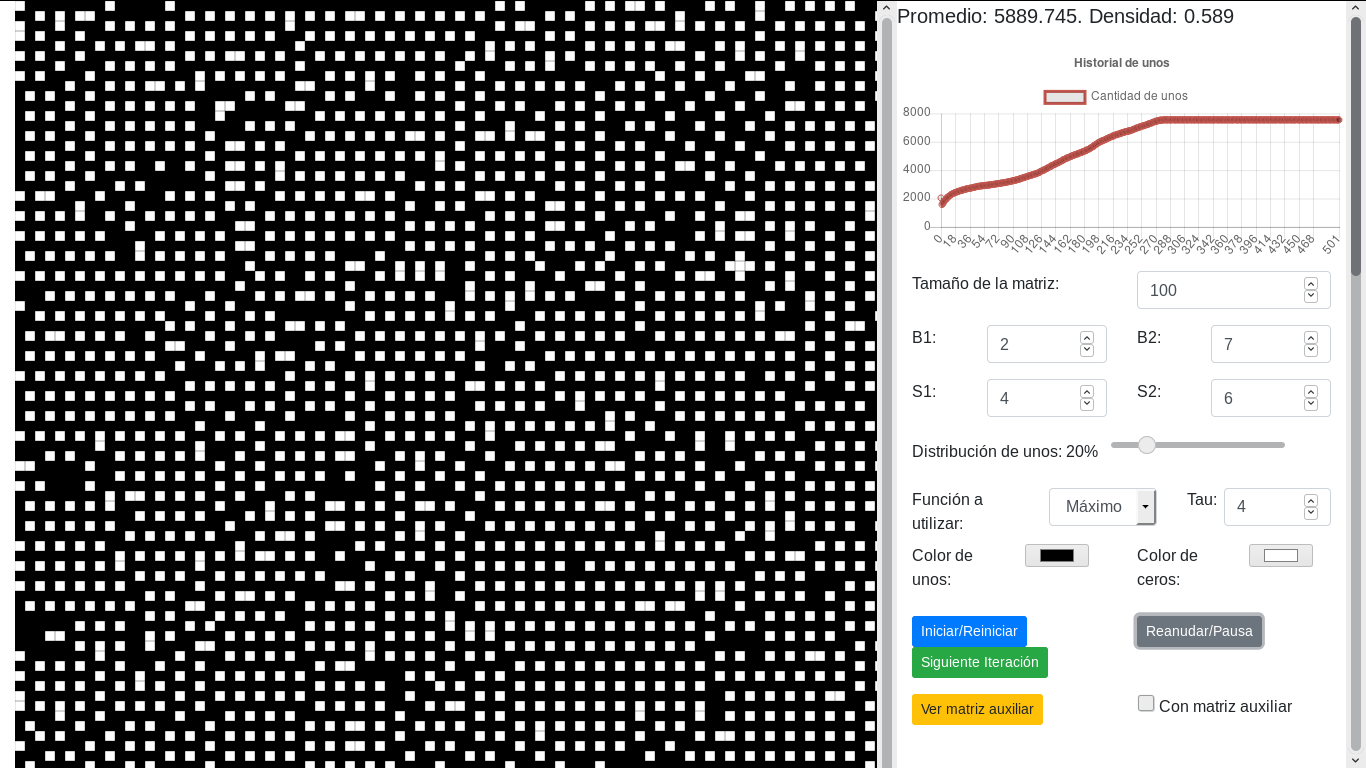
\includegraphics[width=15cm, height=7cm]{./img/2746.png}
 \caption{Resultado tras 100 iteraciones sin matriz auxiliar}
 \label{fig:2746}
\end{center}
\end{figure}
Al aplicar la función de máximo no se llena todo el espacio y se estanca en una cantidad de unos.
\begin{figure}[H]
\begin{center}
 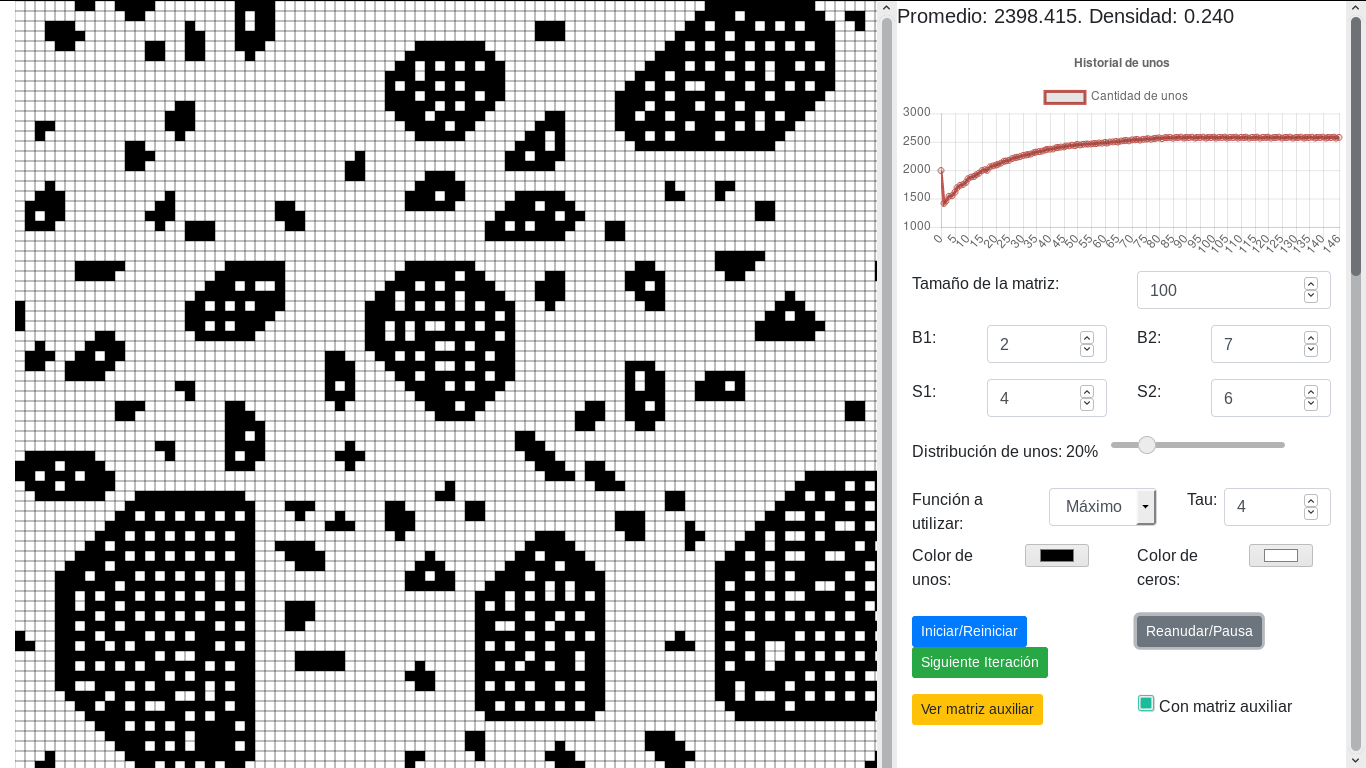
\includegraphics[width=15cm, height=8cm]{./img/2746-max.png}
 \caption{Utilizando la función de máximo}
 \label{fig:2746-max}
\end{center}
\end{figure}
Es importante mencionar que el resultado obtenido al aplicar la función mínimo es muy similar al de máximo pero la matriz auxiliar se invierte.
\begin{figure}[H]
\begin{center}
 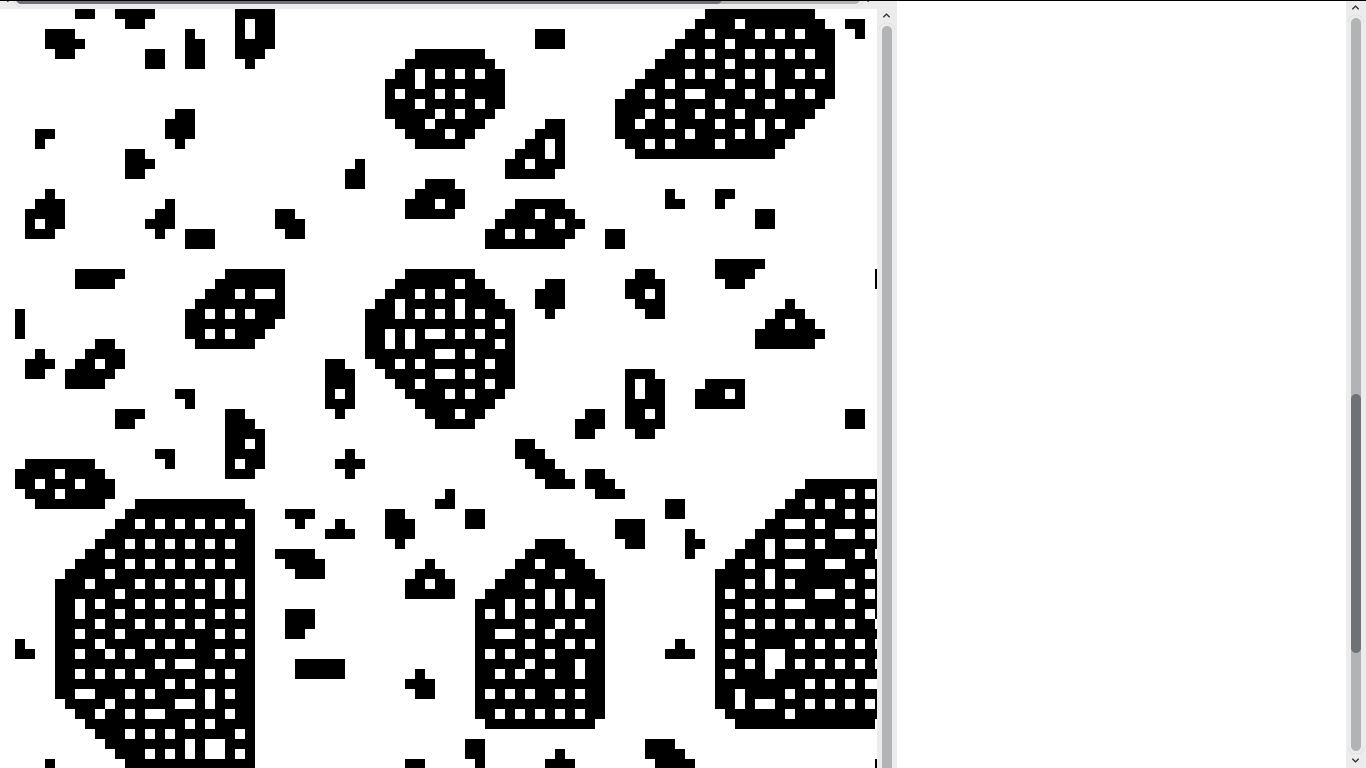
\includegraphics[width=15cm, height=7cm]{./img/2746-max-aux.png}
 \caption{Matriz auxiliar del autómata anterior}
 \label{fig:2746-max-aux}
\end{center}
\end{figure}
La figura \ref{fig:2746-paridad} es el resultado de utilizar la función de paridad en la cual la población decrece bastante rápido hasta quedarse en un solo patrón.
\begin{figure}[H]
\begin{center}
 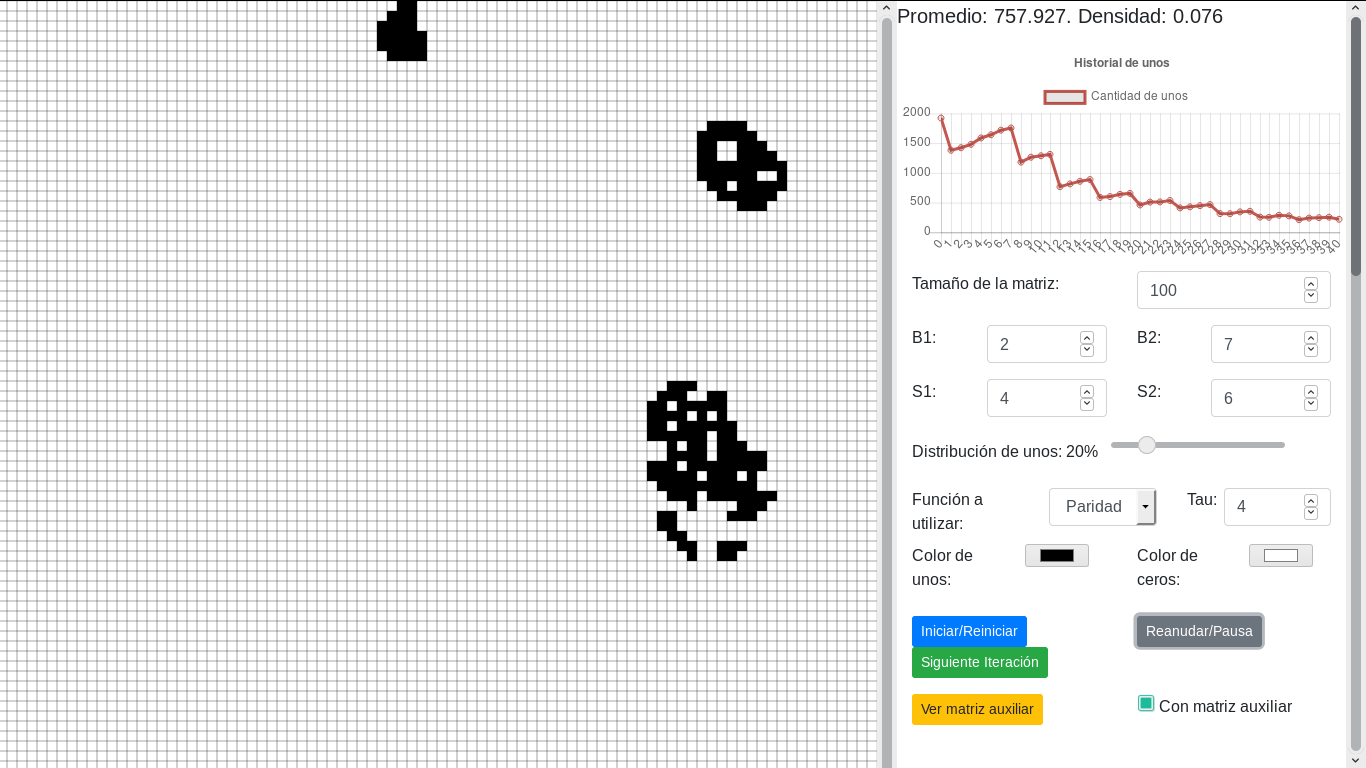
\includegraphics[width=15cm, height=8cm]{./img/2746-paridad.png}
 \caption{Utilizando la función de paridad}
 \label{fig:2746-paridad}
\end{center}
\end{figure}
El comportamiento del automata anterior se puede ver reflejado en la matriz auxiliar que se muestra en la figura \ref{fig:2746-paridad-aux}.
\begin{figure}[H]
\begin{center}
 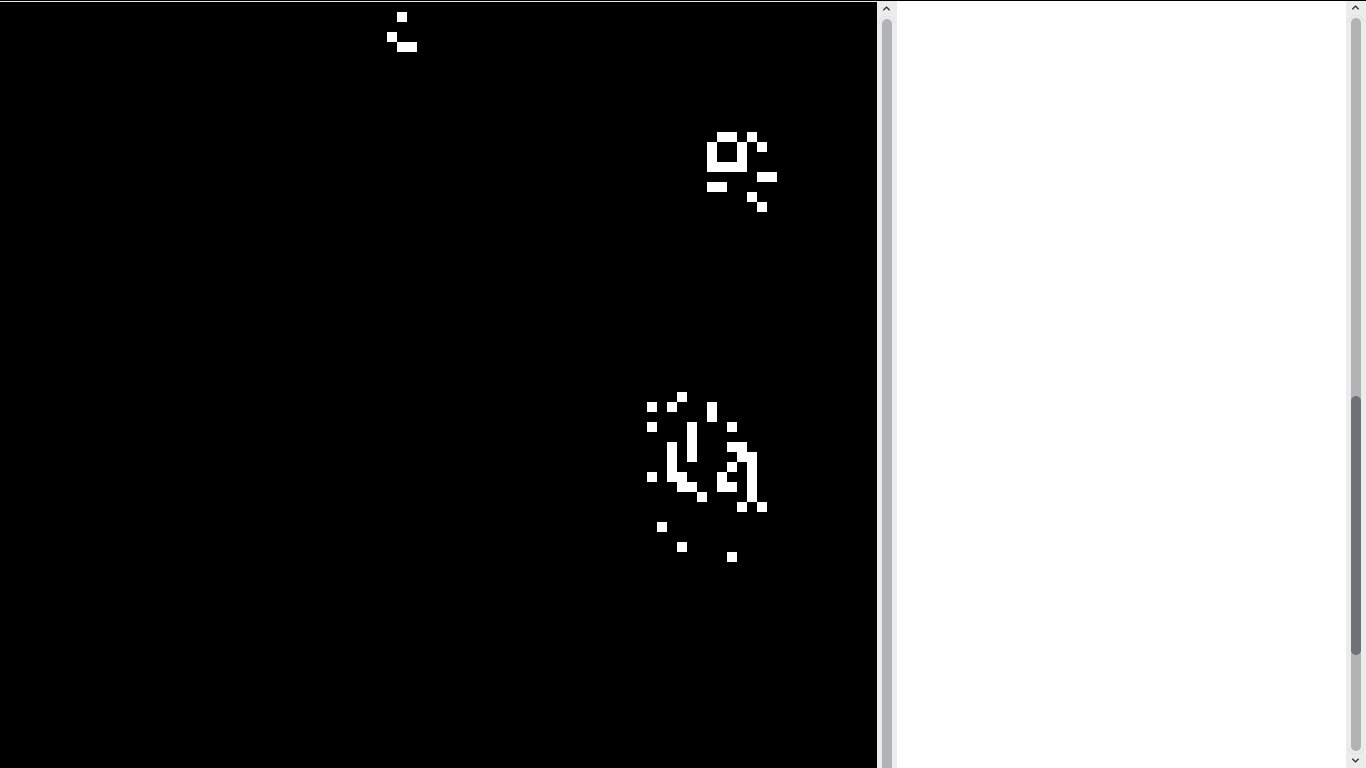
\includegraphics[width=15cm, height=8cm]{./img/2746-paridad-aux.png}
 \caption{Matriz auxiliar del autómata anterior}
 \label{fig:2746-paridad-aux}
\end{center}
\end{figure}

\subsection{Regla: 3 6 3 4. Densidad: 20\%}
El comportamiento de esta regla es similar al anterior pero con una curva de crecimiento más suave.
\begin{figure}[H]
\begin{center}
 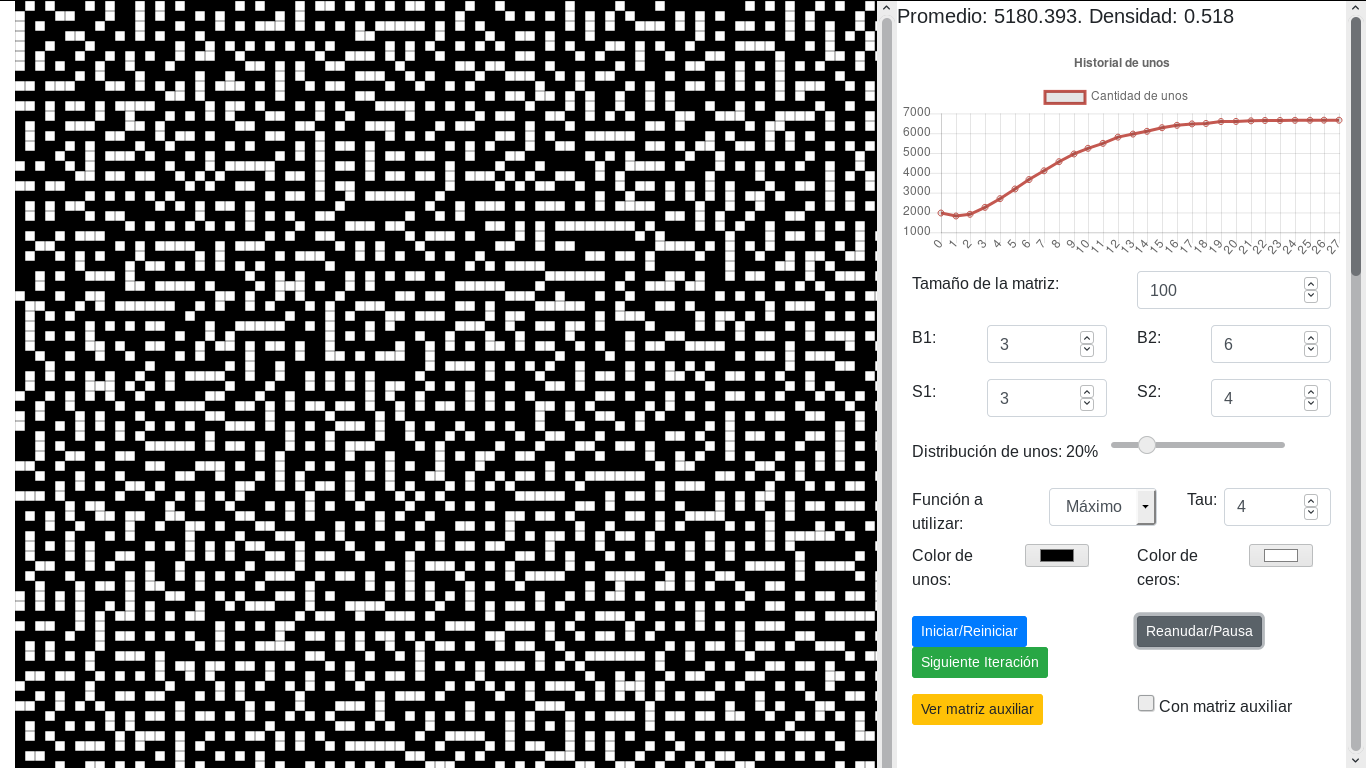
\includegraphics[width=15cm, height=8cm]{./img/3634.png}
 \caption{Resultado tras 100 iteraciones sin matriz auxiliar}
 \label{fig:3634}
\end{center}
\end{figure}
Al utilizar la función de mínimo que se observa en la figura \ref{fig:3634-min} se llega al mismo resultado pero con algunas perturbaciones al inicio de su crecimiento.
\begin{figure}[H]
\begin{center}
 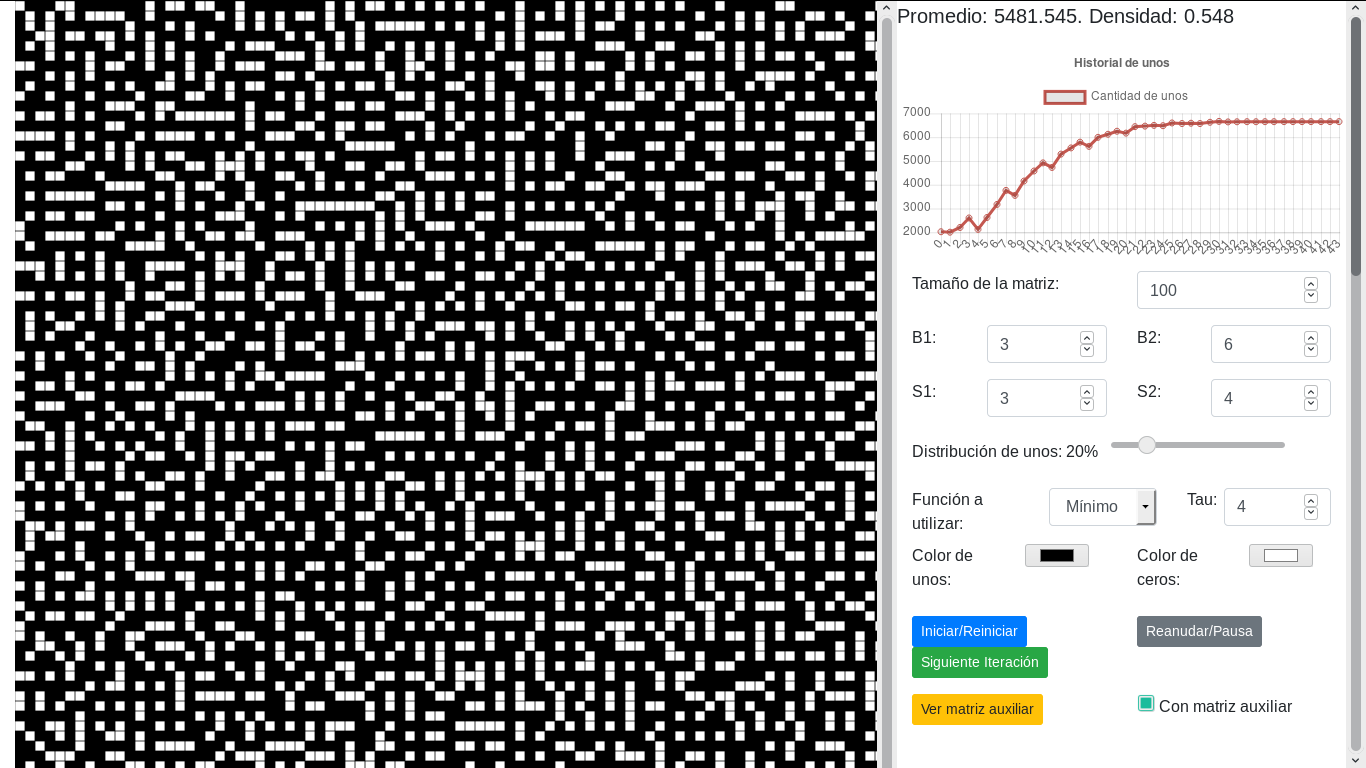
\includegraphics[width=15cm, height=8cm]{./img/3634-min.png}
 \caption{Utilizando la función de mínimo}
 \label{fig:3634-min}
\end{center}
\end{figure}

Si se utiliza una función de máximo se obtiene un resultado similar pero invirtiendo los colores de la matriz auxiliar que se observa en la figura \ref{fig:3634-min-aux}.

\begin{figure}[H]
\begin{center}
 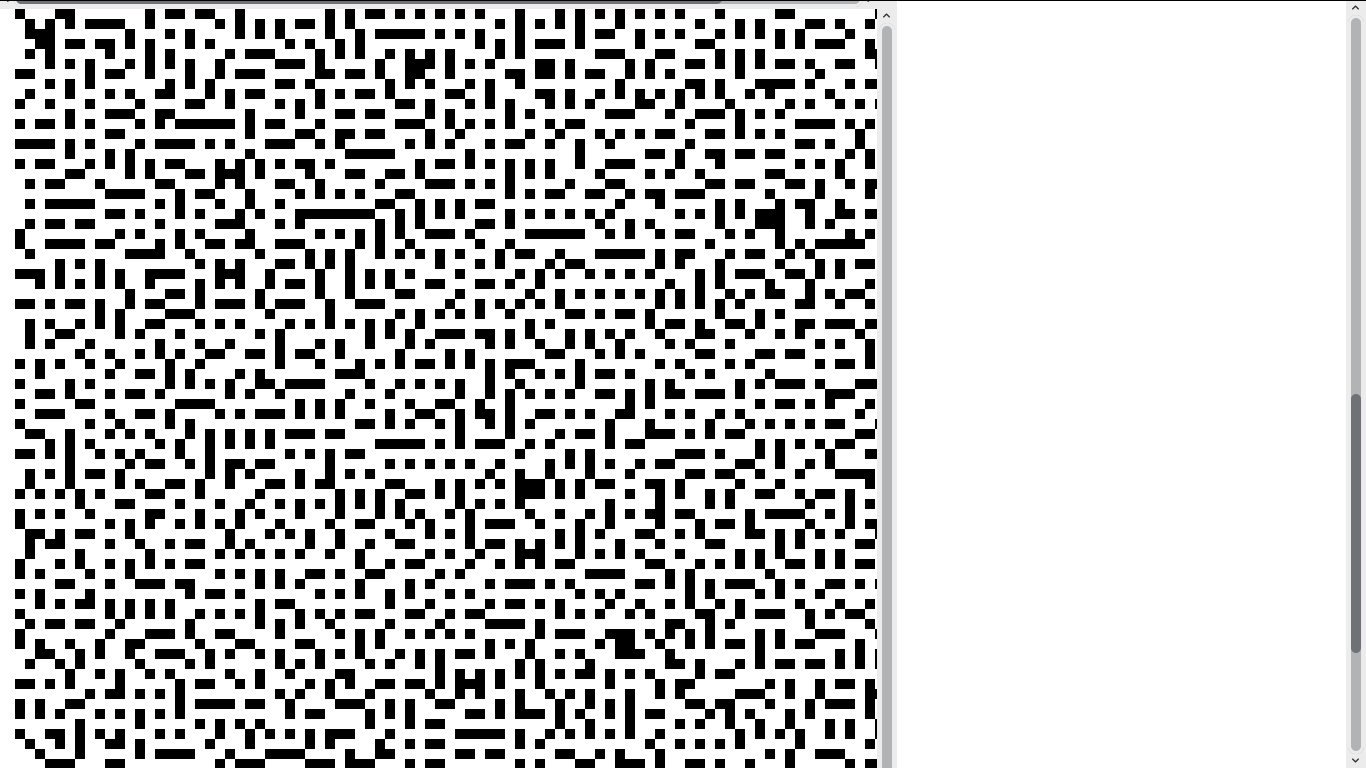
\includegraphics[width=15cm, height=8cm]{./img/3634-min-aux.png}
 \caption{Matriz auxiliar del autómata anterior}
 \label{fig:3634-min-aux}
\end{center}
\end{figure}
La función de paridad es la que provoca el comportamiento más inestable ya que a pesar de que crece como en los ejemplos anteriores su población oscila a lo largo de un rango de valores 
\begin{figure}[H]
\begin{center}
 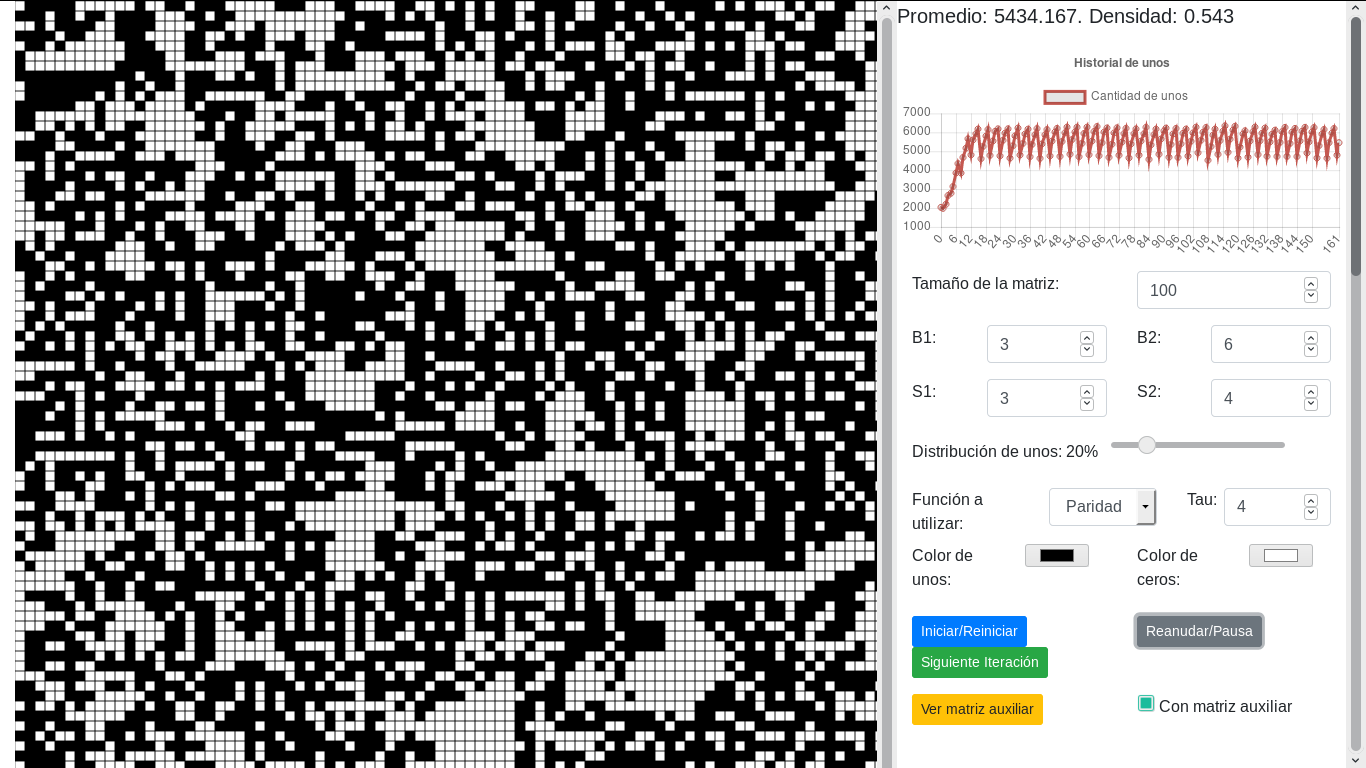
\includegraphics[width=15cm, height=8cm]{./img/3634-paridad.png}
 \caption{Utilizando la función de paridad}
 \label{fig:3634-paridad}
\end{center}
\end{figure}
El comportamiento oscilatorio se observa en la matriz auxiliar ya que esta parece solo cambiar de colores una y otra vez.
\begin{figure}[H]
\begin{center}
 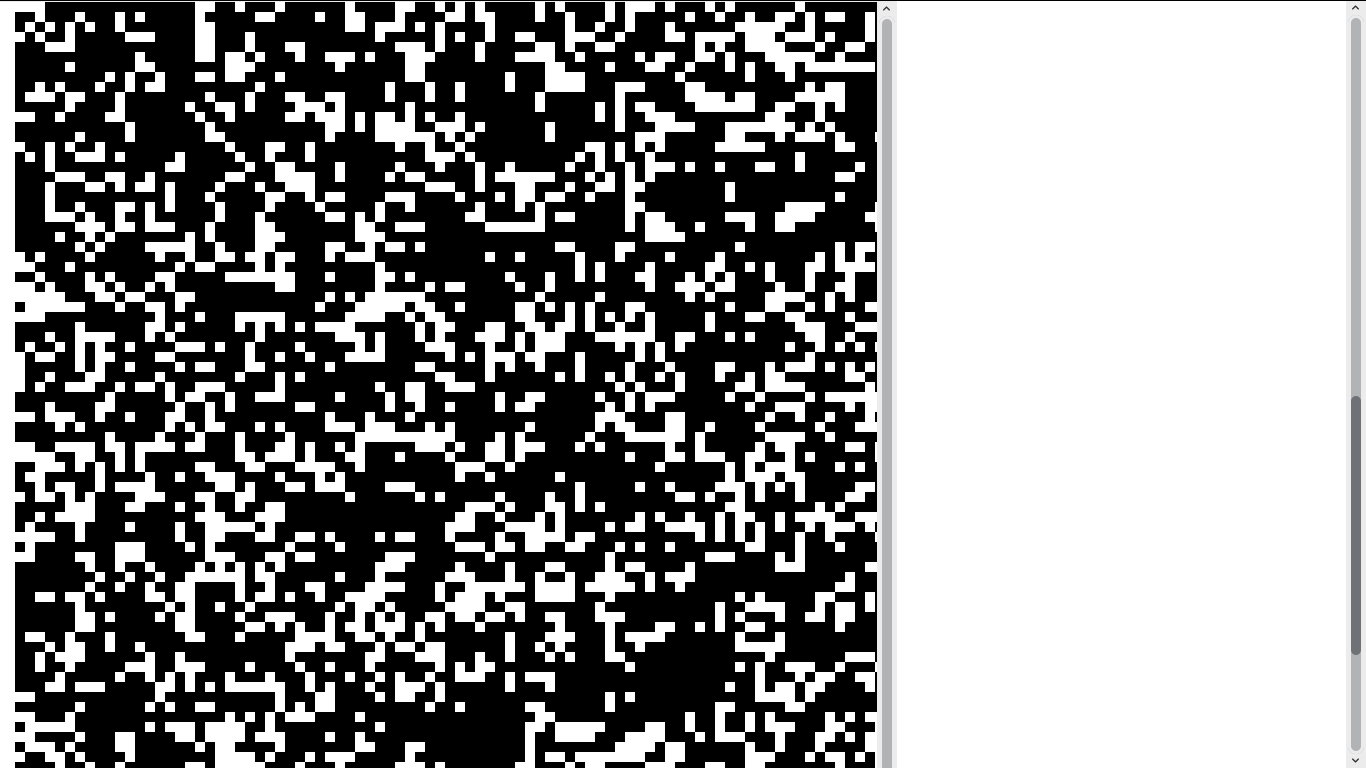
\includegraphics[width=15cm, height=8cm]{./img/3634-paridad-aux.png}
 \caption{Matriz auxiliar del autómata anterior}
 \label{fig:3634-paridad-aux}
\end{center}
\end{figure}

\subsection{Regla: 1 6 1 6. Densidad: 10\%}
El comportamiento de esta regla se tiende a estabilizar bastante rápido y formar una estructura que ya no cambia.

\begin{figure}[H]
\begin{center}
 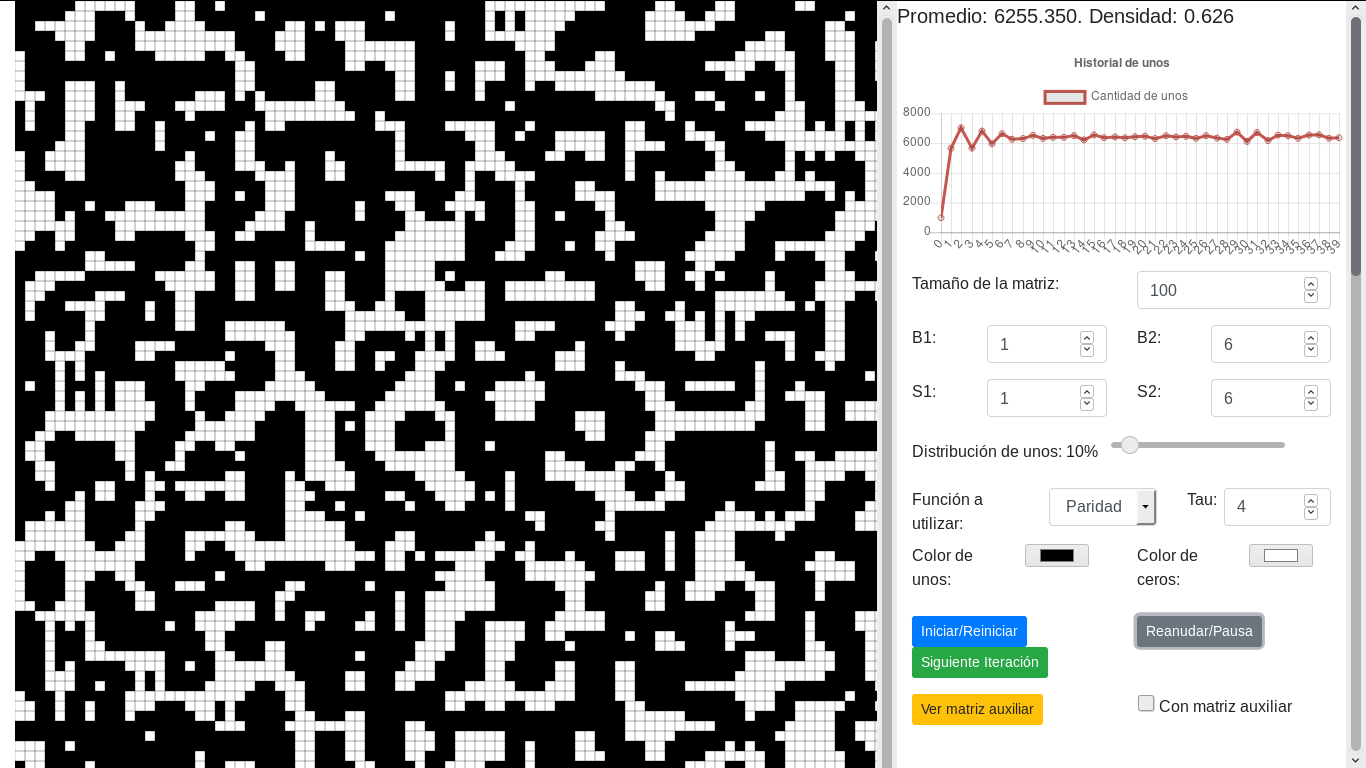
\includegraphics[width=15cm, height=8cm]{./img/1616.png}
 \caption{Resultado tras 100 iteraciones sin matriz auxiliar}
 \label{fig:1616}
\end{center}
\end{figure}

\begin{figure}[H]
\begin{center}
 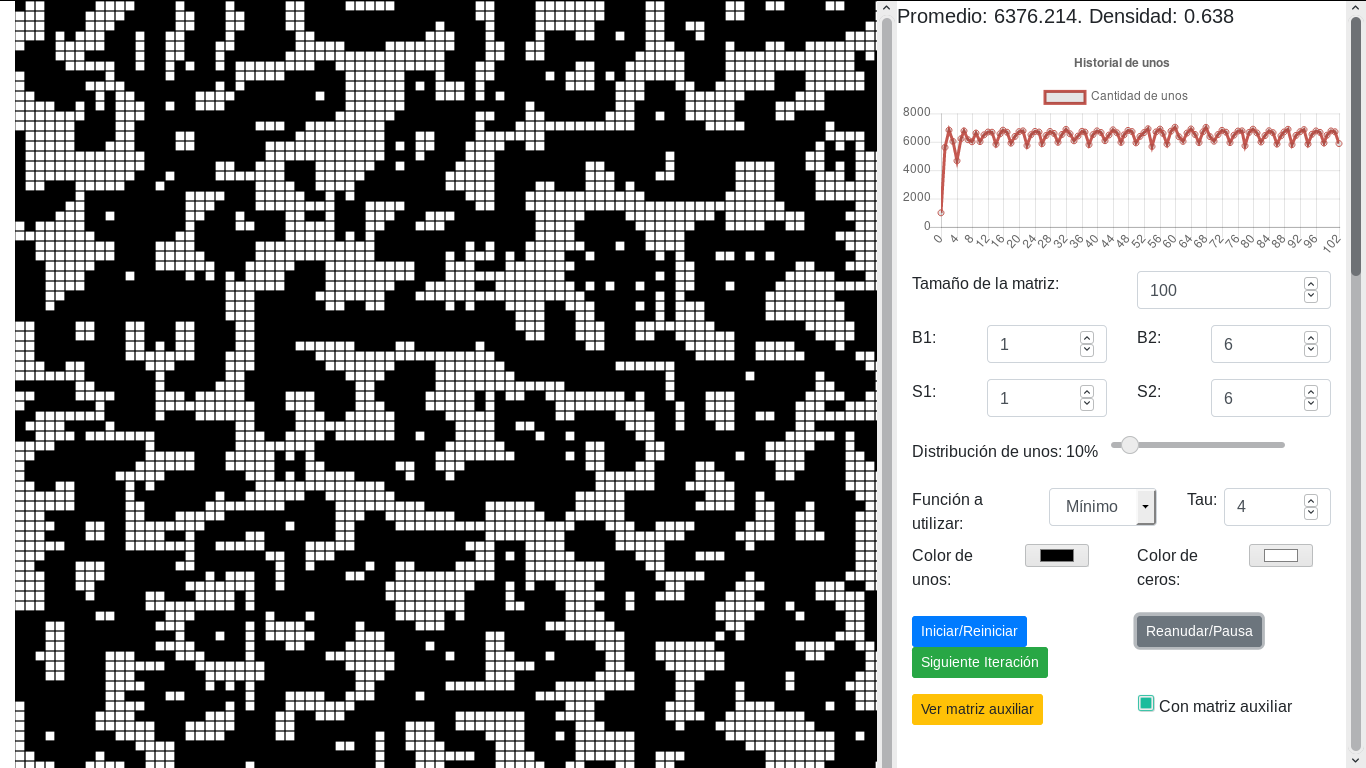
\includegraphics[width=15cm, height=8cm]{./img/1616-min.png}
 \caption{Utilizando la función de mínimo}
 \label{fig:1616-min}
\end{center}
\end{figure}

\begin{figure}[H]
\begin{center}
 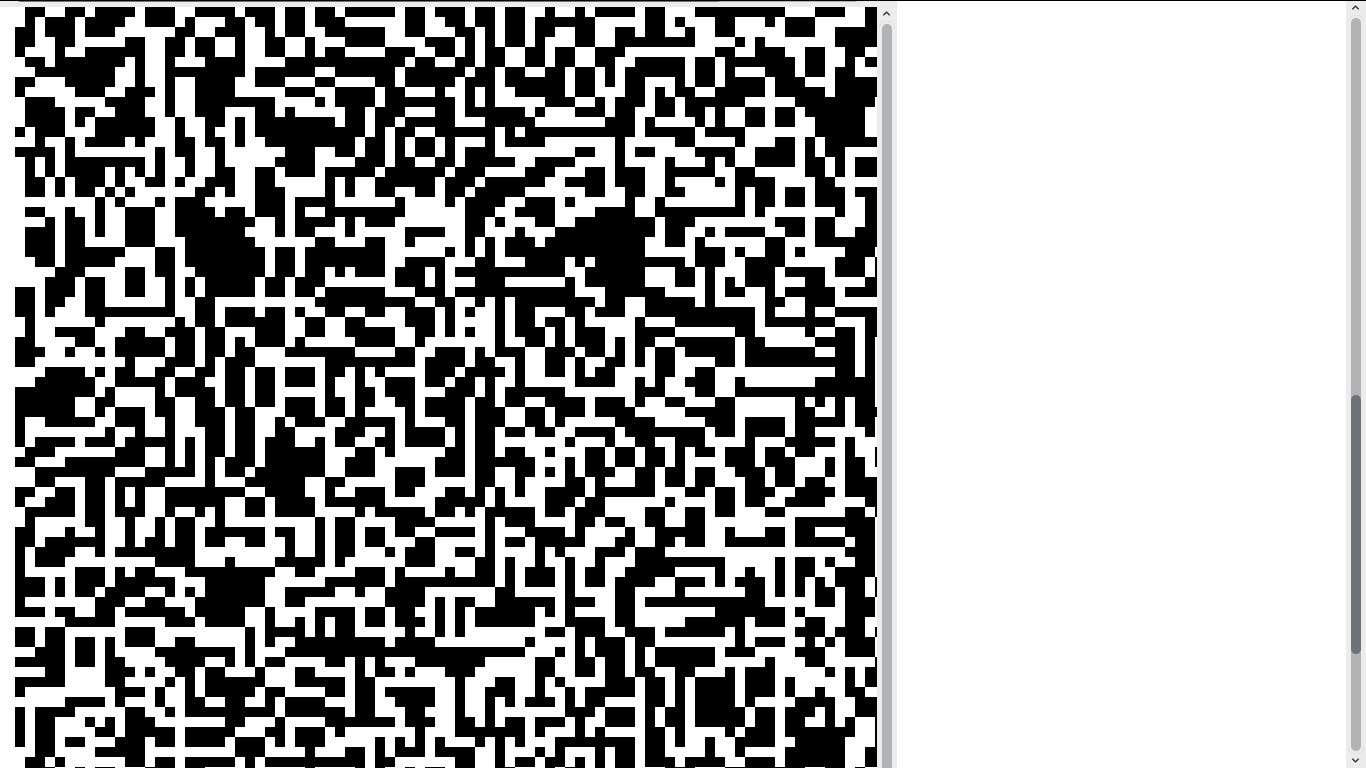
\includegraphics[width=15cm, height=8cm]{./img/1616-min-aux.png}
 \caption{Matriz auxiliar del autómata anterior}
 \label{fig:1616-min-aux}
\end{center}
\end{figure}

\begin{figure}[H]
\begin{center}
 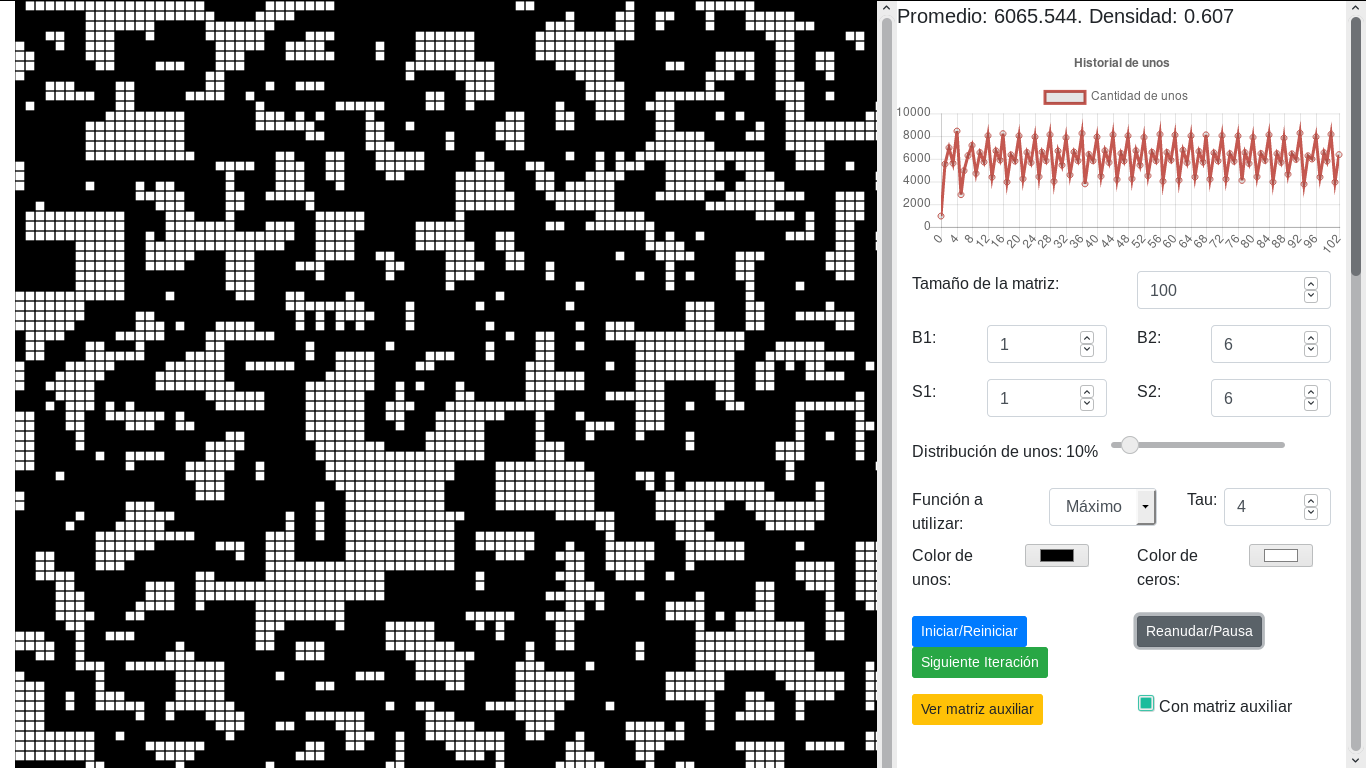
\includegraphics[width=15cm, height=8cm]{./img/1616-max.png}
 \caption{Utilizando la función de máximo}
 \label{fig:1616-max}
\end{center}
\end{figure}

\begin{figure}[H]
\begin{center}
 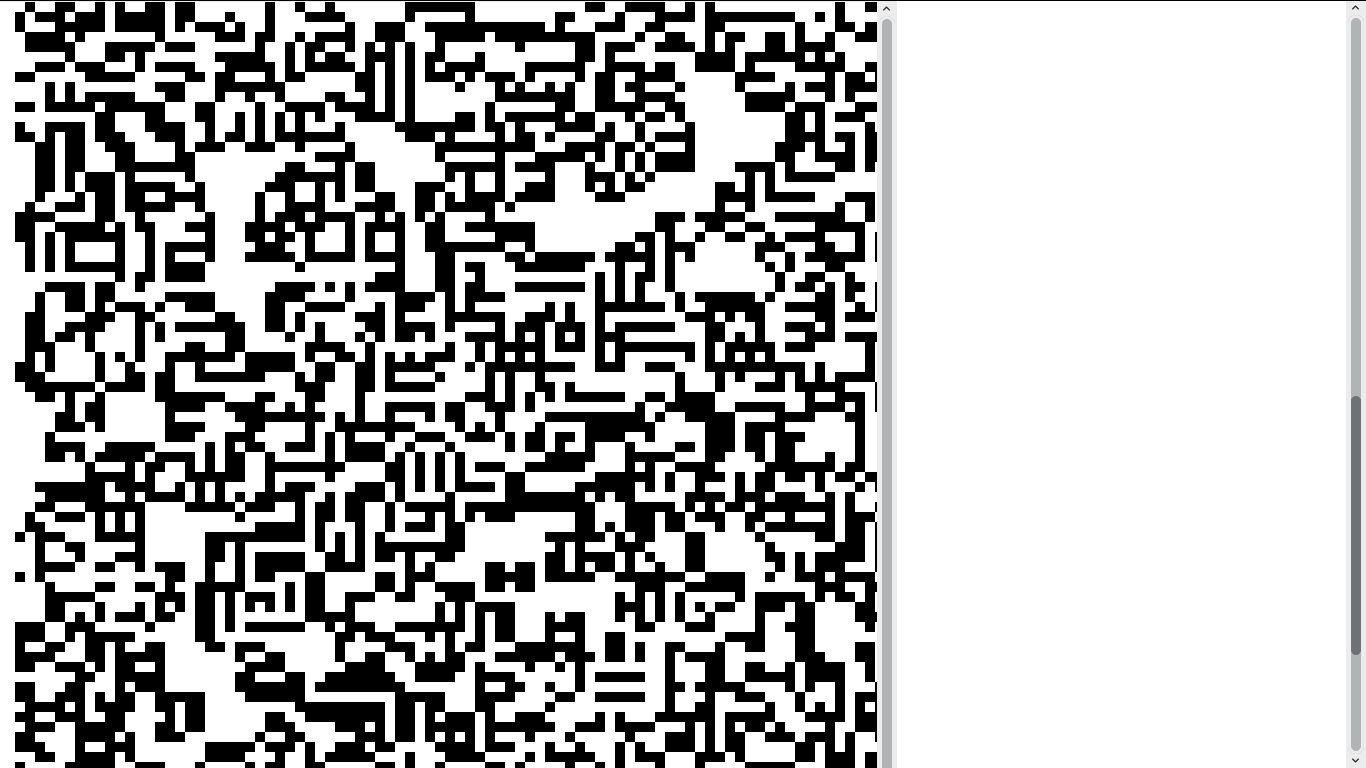
\includegraphics[width=15cm, height=8cm]{./img/1616-max-aux.png}
 \caption{Matriz auxiliar del autómata anterior}
 \label{fig:1616-max-aux}
\end{center}
\end{figure}

\begin{figure}[H]
\begin{center}
 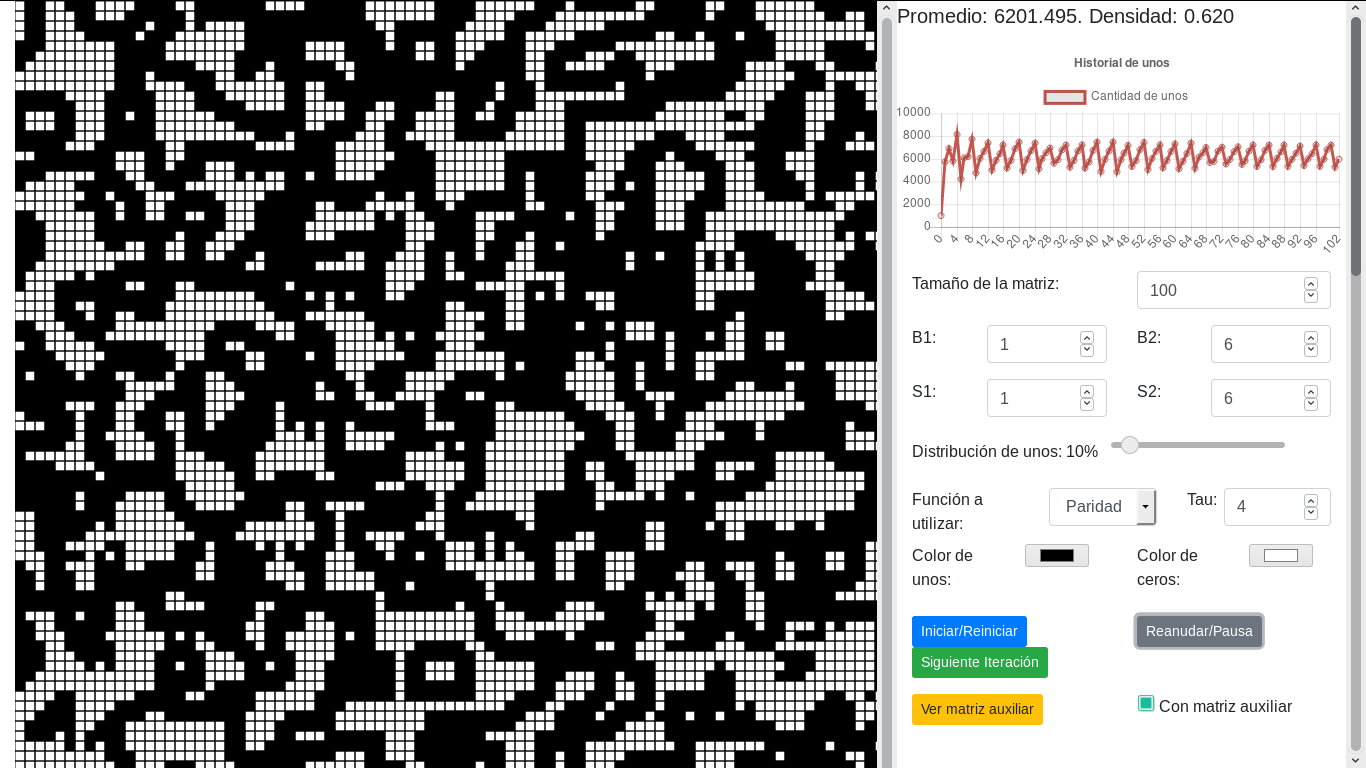
\includegraphics[width=15cm, height=8cm]{./img/1616-paridad.png}
 \caption{Utilizando la función de paridad}
 \label{fig:1616-paridad}
\end{center}
\end{figure}

\begin{figure}[H]
\begin{center}
 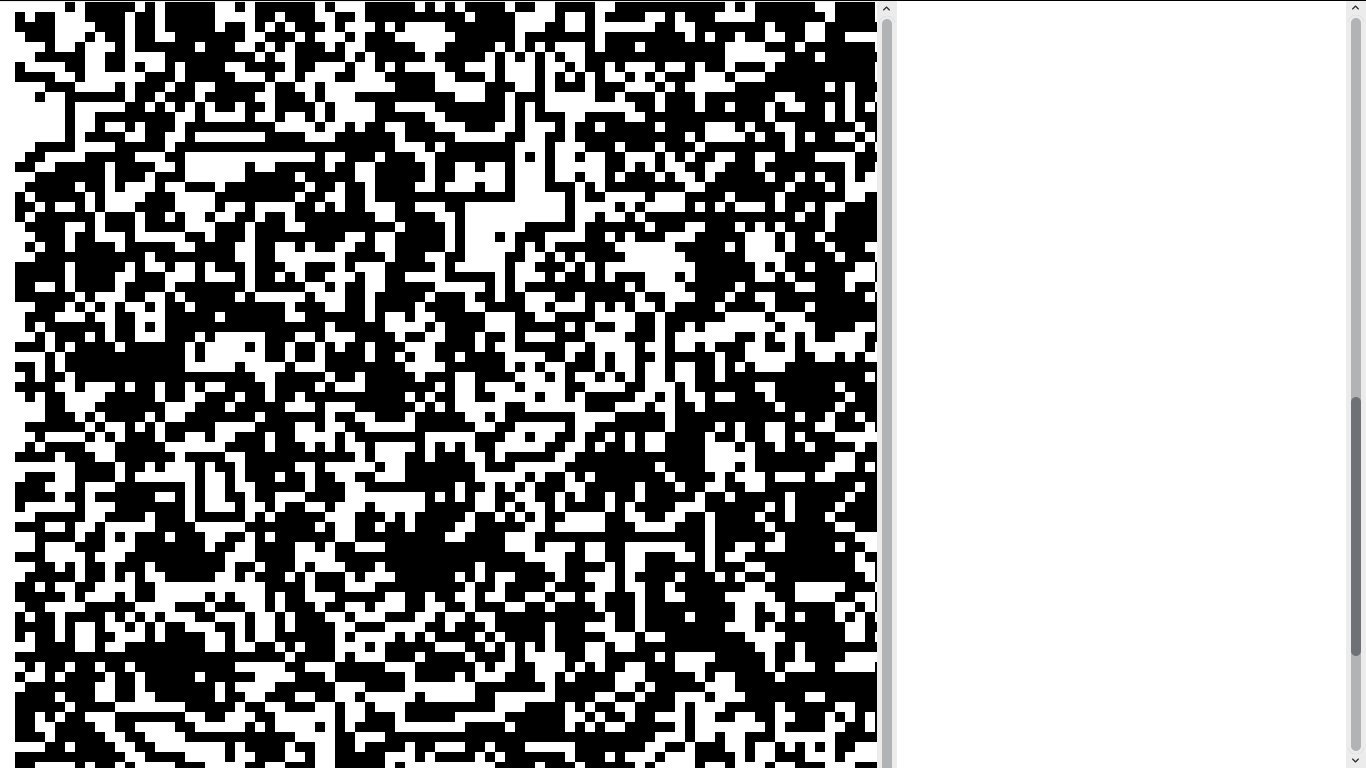
\includegraphics[width=15cm, height=8cm]{./img/1616-paridad-aux.png}
 \caption{Matriz auxiliar del autómata anterior}
 \label{fig:1616-paridad-aux}
\end{center}
\end{figure}
Con esta regla y utilizando las tres funciones se obtiene el mismo resultado, sin embargo, el comportamiento de la cantidad de unos es diferente. Para la función de máximo se tiene el comportamiento más oscilatorio, después le sigue la función de paridad y por ultimo la función de mínimo. 

\subsection{Regla: 3 3 1 8. Densidad: 10\%}
El comportamiento de esta regla oscila bastante y llega a un punto en el que parece que solo cambia los colores de las células.
\begin{figure}[H]
\begin{center}
 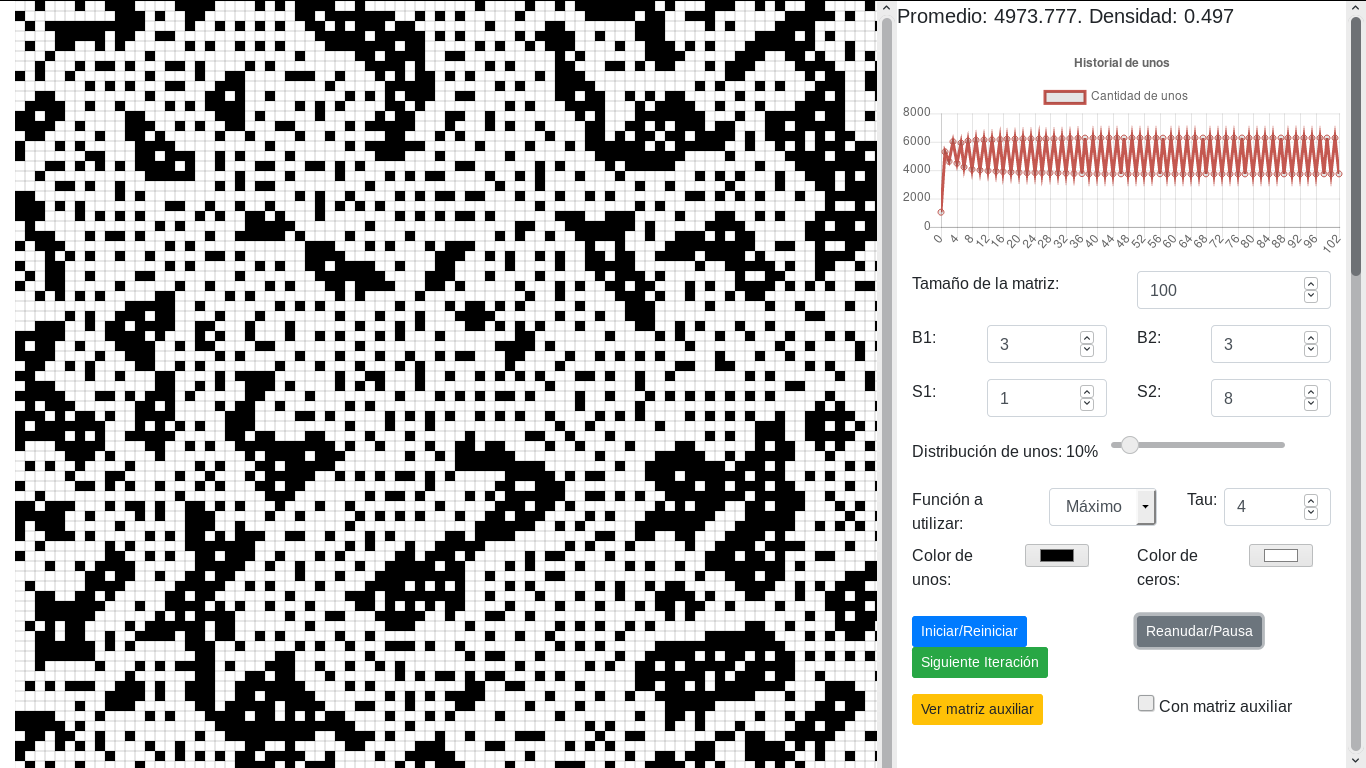
\includegraphics[width=15cm, height=8cm]{./img/3318.png}
 \caption{Resultado tras 100 iteraciones sin matriz auxiliar}
 \label{fig:3318}
\end{center}
\end{figure}
Para la regla de mínimo se tiene un comportamiento extraño en el cual en lugar de aumentar la población y estabilizarse ocurre lo contrario hasta quedar con solo algunos patrones en la matriz.
\begin{figure}[H]
\begin{center}
 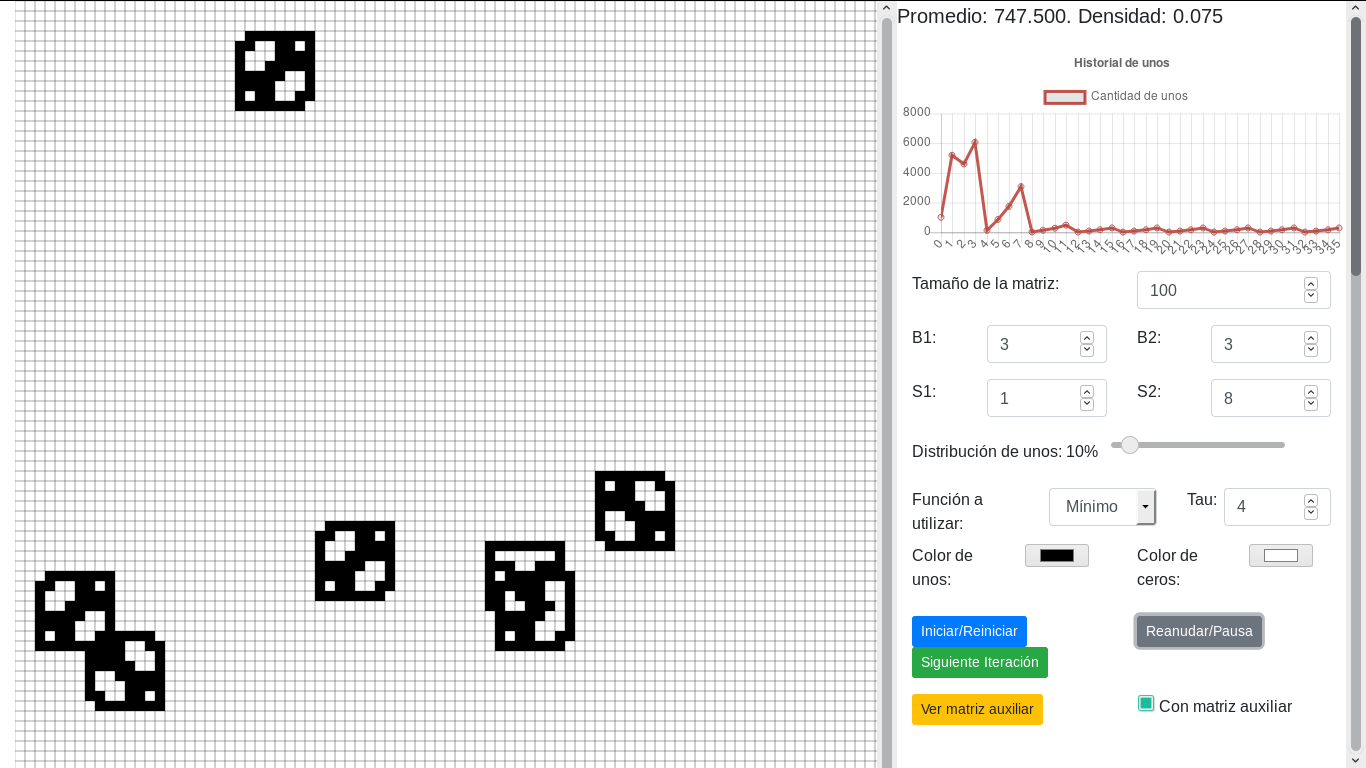
\includegraphics[width=15cm, height=8cm]{./img/3318-min.png}
 \caption{Utilizando la función de mínimo}
 \label{fig:3318-min}
\end{center}
\end{figure}

\begin{figure}[H]
\begin{center}
 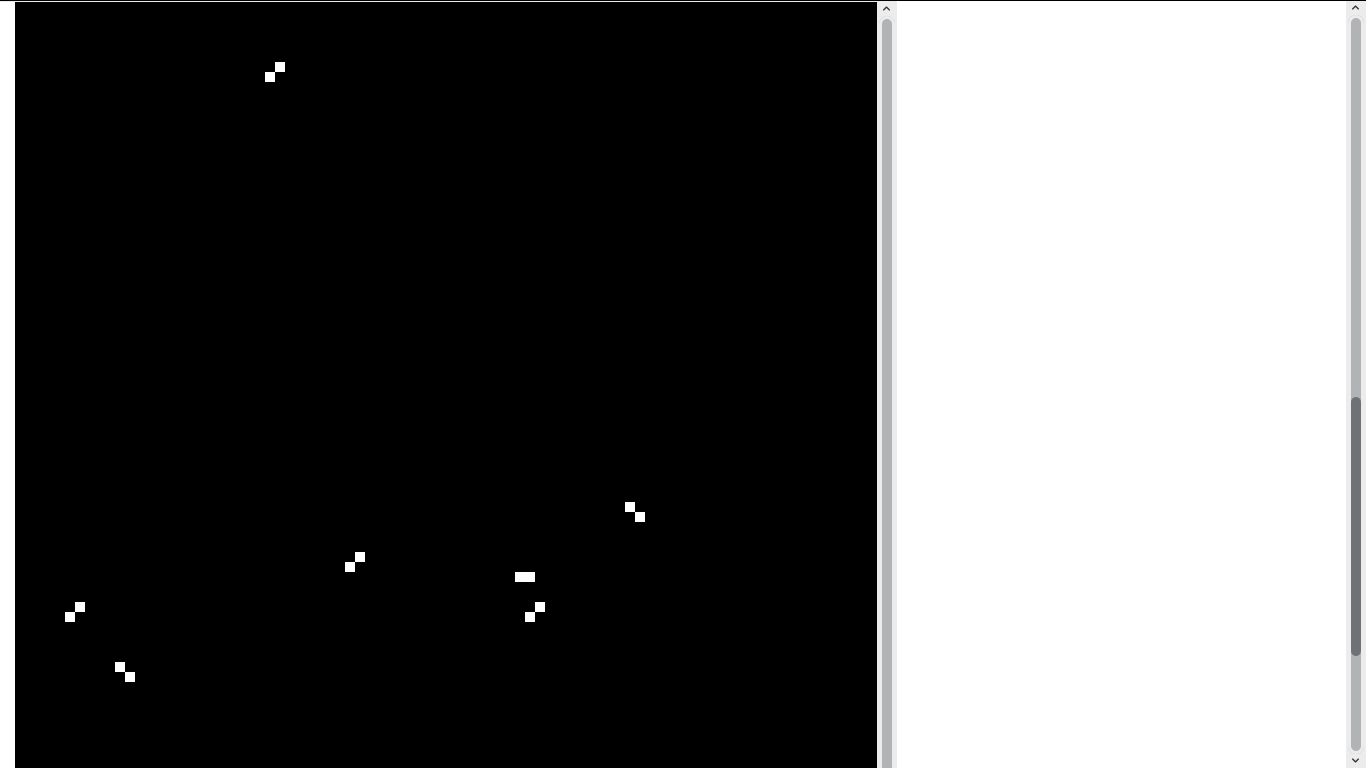
\includegraphics[width=15cm, height=8cm]{./img/3318-min-aux.png}
 \caption{Matriz auxiliar del autómata anterior}
 \label{fig:3318-min-aux}
\end{center}
\end{figure}
Al aplicar la función máximo se reduce la cantidad de oscilaciones que se tienen a lo largo de las iteraciones.
\begin{figure}[H]
\begin{center}
 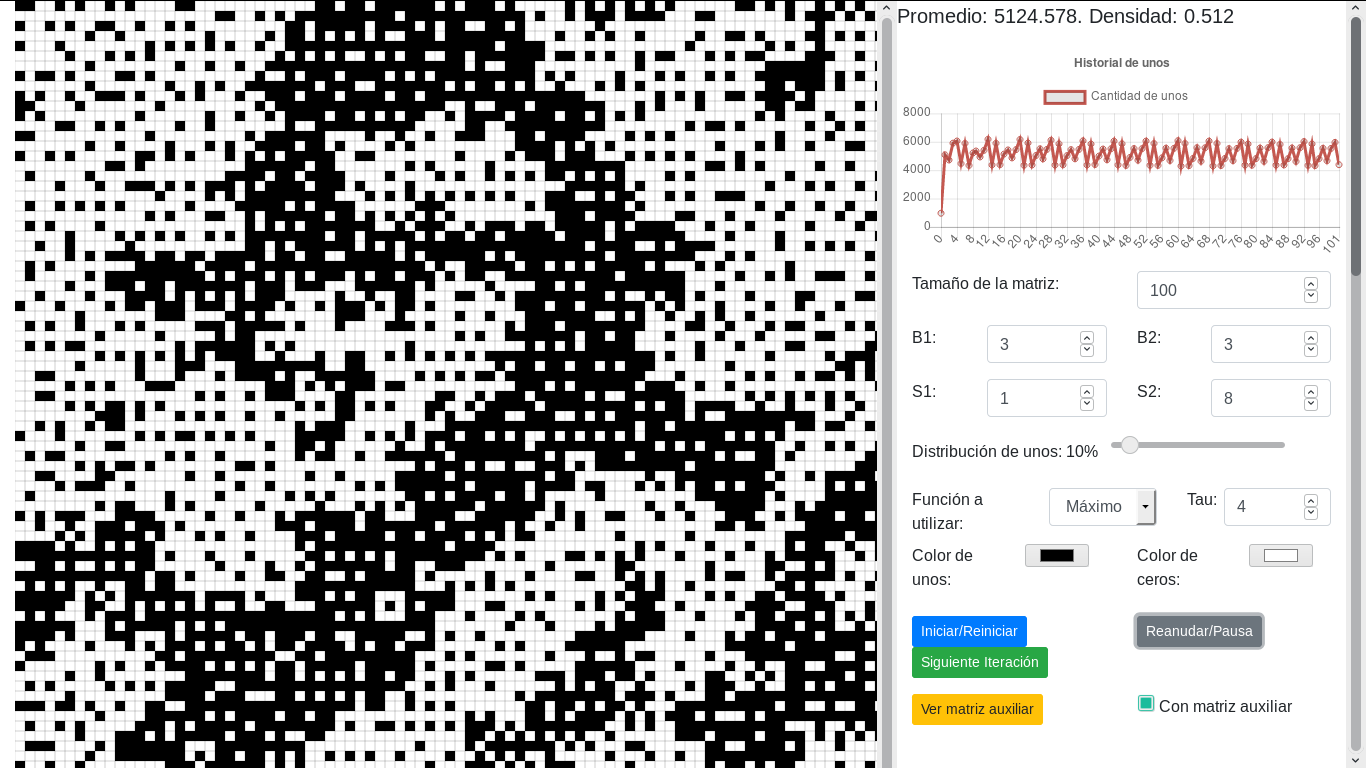
\includegraphics[width=15cm, height=8cm]{./img/3318-max.png}
 \caption{Utilizando la función de máximo}
 \label{fig:3318-max}
\end{center}
\end{figure}

\begin{figure}[H]
\begin{center}
 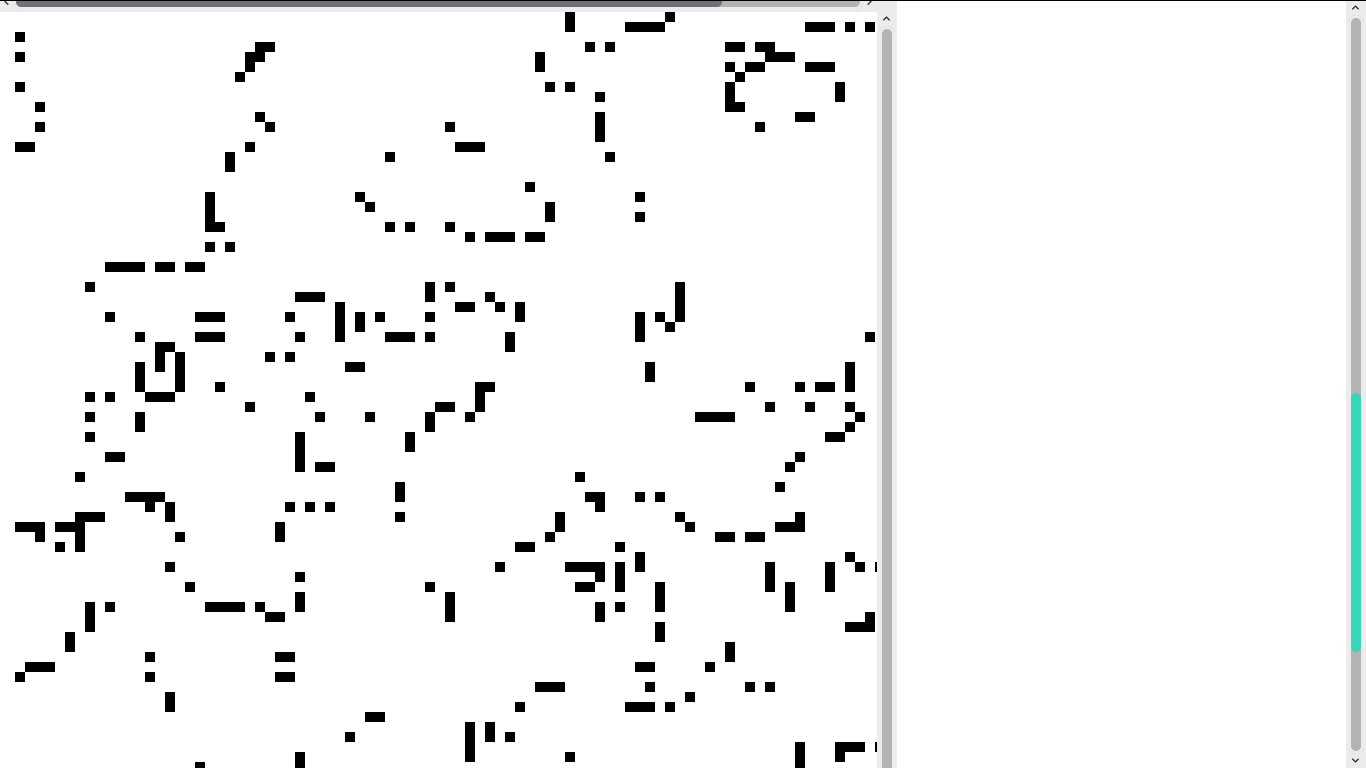
\includegraphics[width=15cm, height=8cm]{./img/3318-max-aux.png}
 \caption{Matriz auxiliar del autómata anterior}
 \label{fig:3318-max-aux}
\end{center}
\end{figure}
En contraste con la función máximo se tiene lo contrario, en esta las oscilaciones son mayores.
\begin{figure}[H]
\begin{center}
 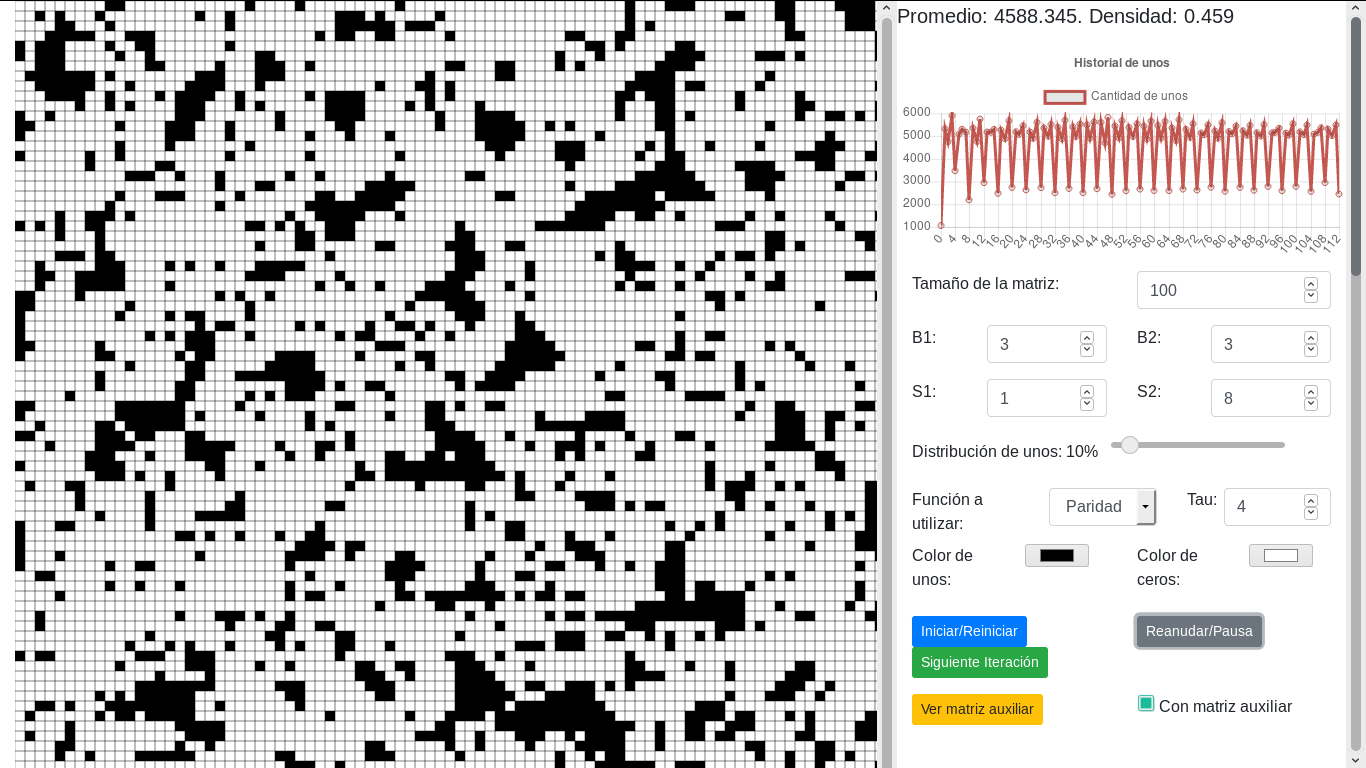
\includegraphics[width=15cm, height=8cm]{./img/3318-paridad.png}
 \caption{Utilizando la función de paridad}
 \label{fig:3318-paridad}
\end{center}
\end{figure}

\begin{figure}[H]
\begin{center}
 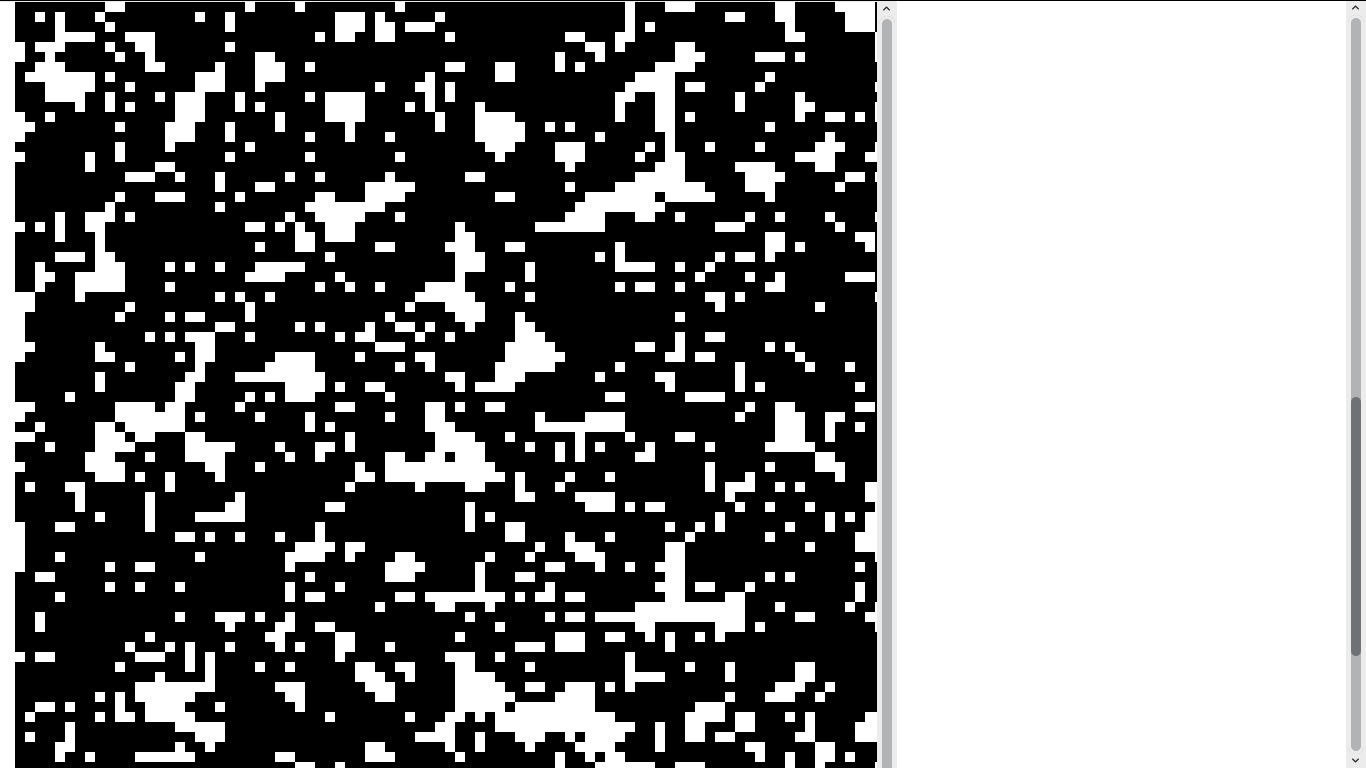
\includegraphics[width=15cm, height=8cm]{./img/3318-paridad-aux.png}
 \caption{Matriz auxiliar del autómata anterior}
 \label{fig:3318-paridad-aux}
\end{center}
\end{figure}

\subsection{Regla: 3 3 1 7. Densidad: 5\%}

\begin{figure}[H]
\begin{center}
 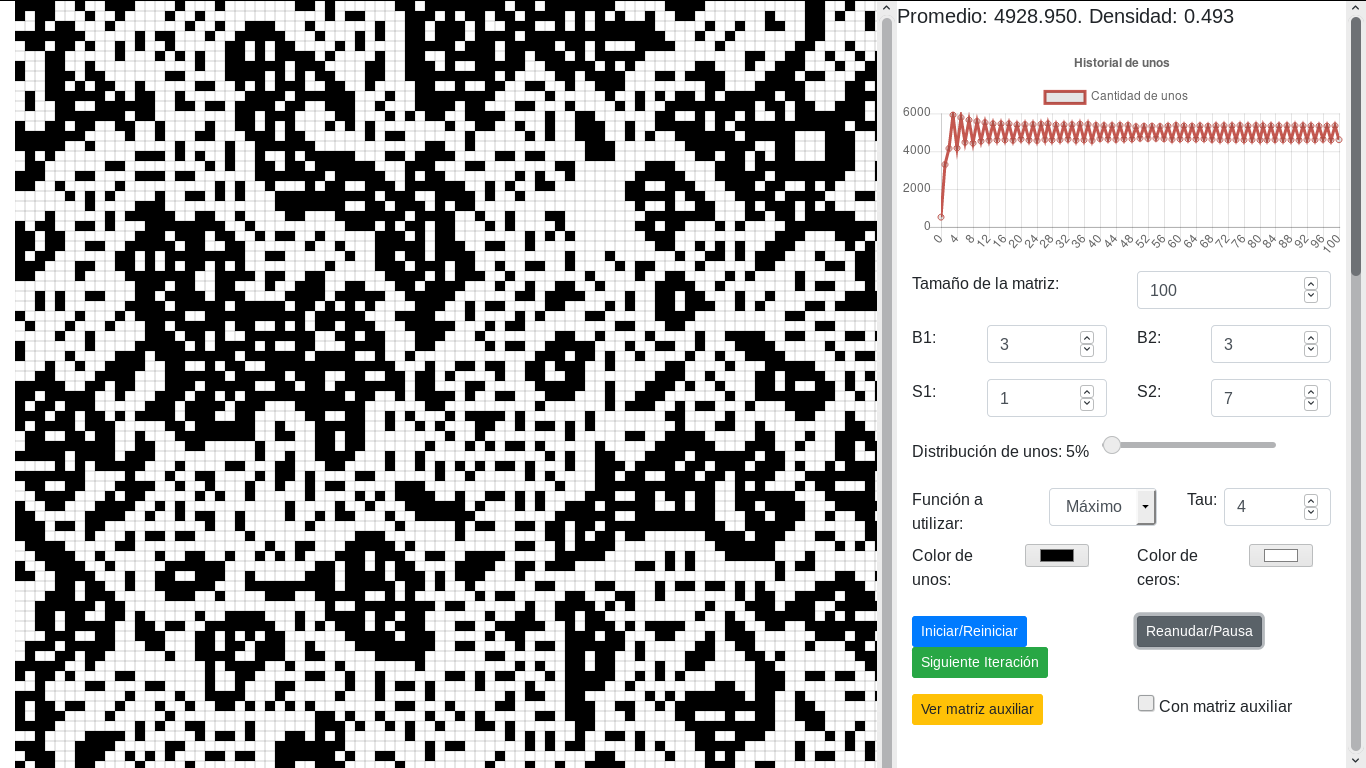
\includegraphics[width=15cm, height=8cm]{./img/3317.png}
 \caption{Resultado tras 100 iteraciones sin matriz auxiliar}
 \label{fig:3317}
\end{center}
\end{figure}

\begin{figure}[H]
\begin{center}
 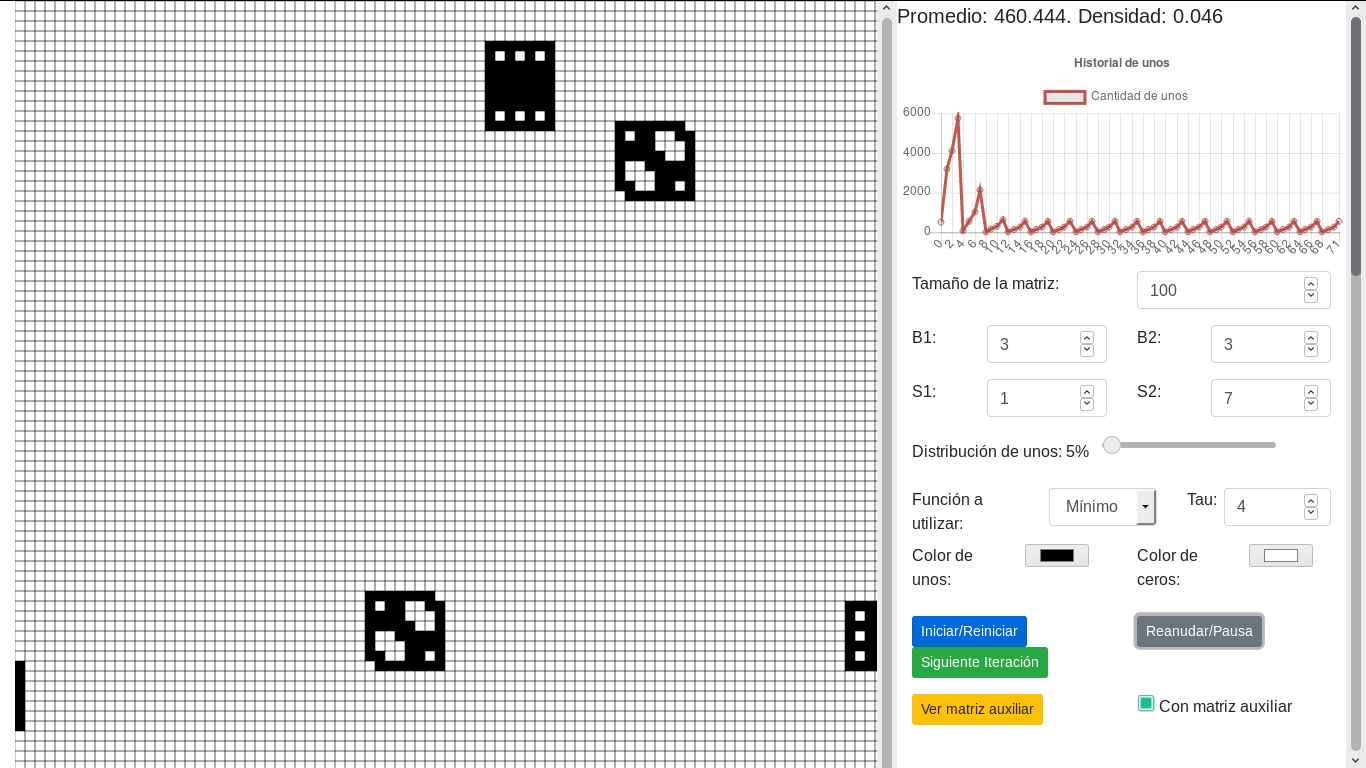
\includegraphics[width=15cm, height=8cm]{./img/3317-min.png}
 \caption{Utilizando la función de mínimo}
 \label{fig:3317-min}
\end{center}
\end{figure}

\begin{figure}[H]
\begin{center}
 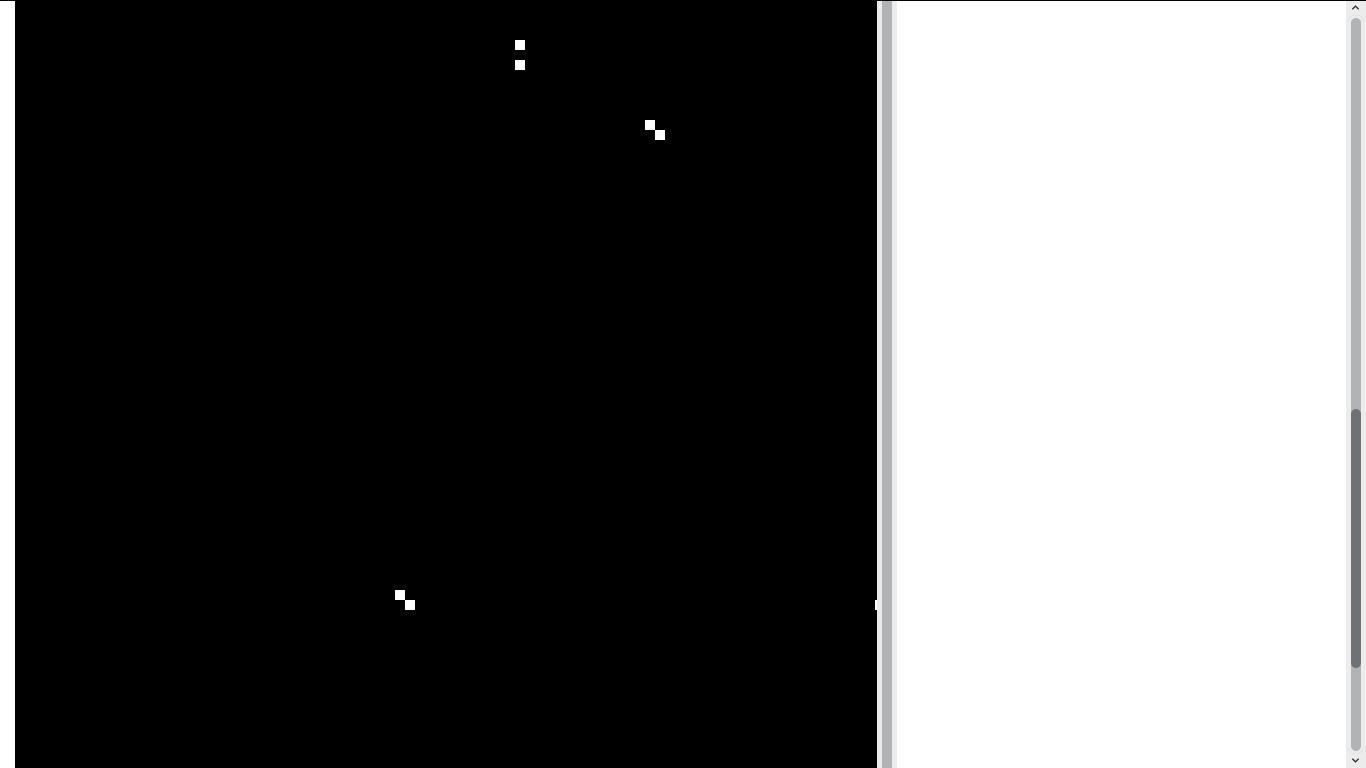
\includegraphics[width=15cm, height=8cm]{./img/3317-min-aux.png}
 \caption{Matriz auxiliar del autómata anterior}
 \label{fig:3317-min-aux}
\end{center}
\end{figure}

\begin{figure}[H]
\begin{center}
 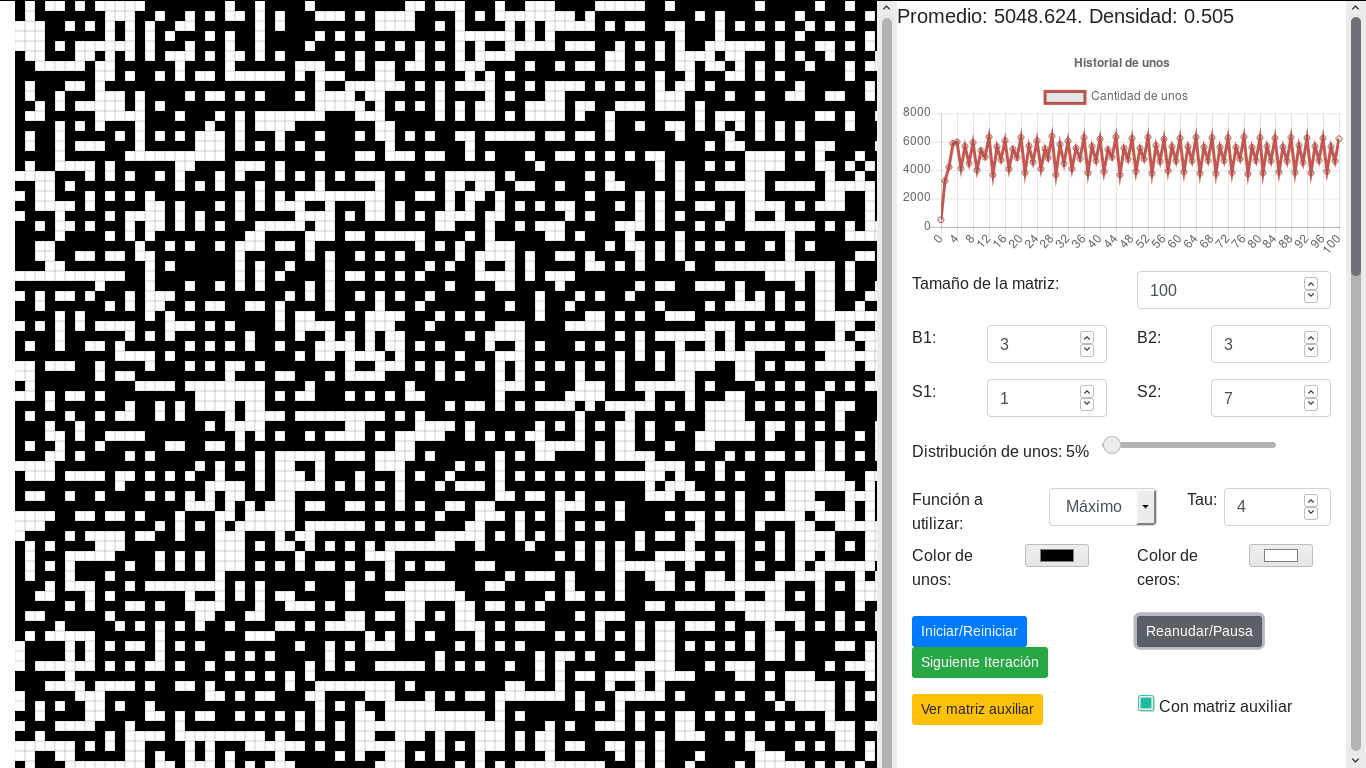
\includegraphics[width=15cm, height=8cm]{./img/3317-max.png}
 \caption{Utilizando la función de máximo}
 \label{fig:3317-max}
\end{center}
\end{figure}

\begin{figure}[H]
\begin{center}
 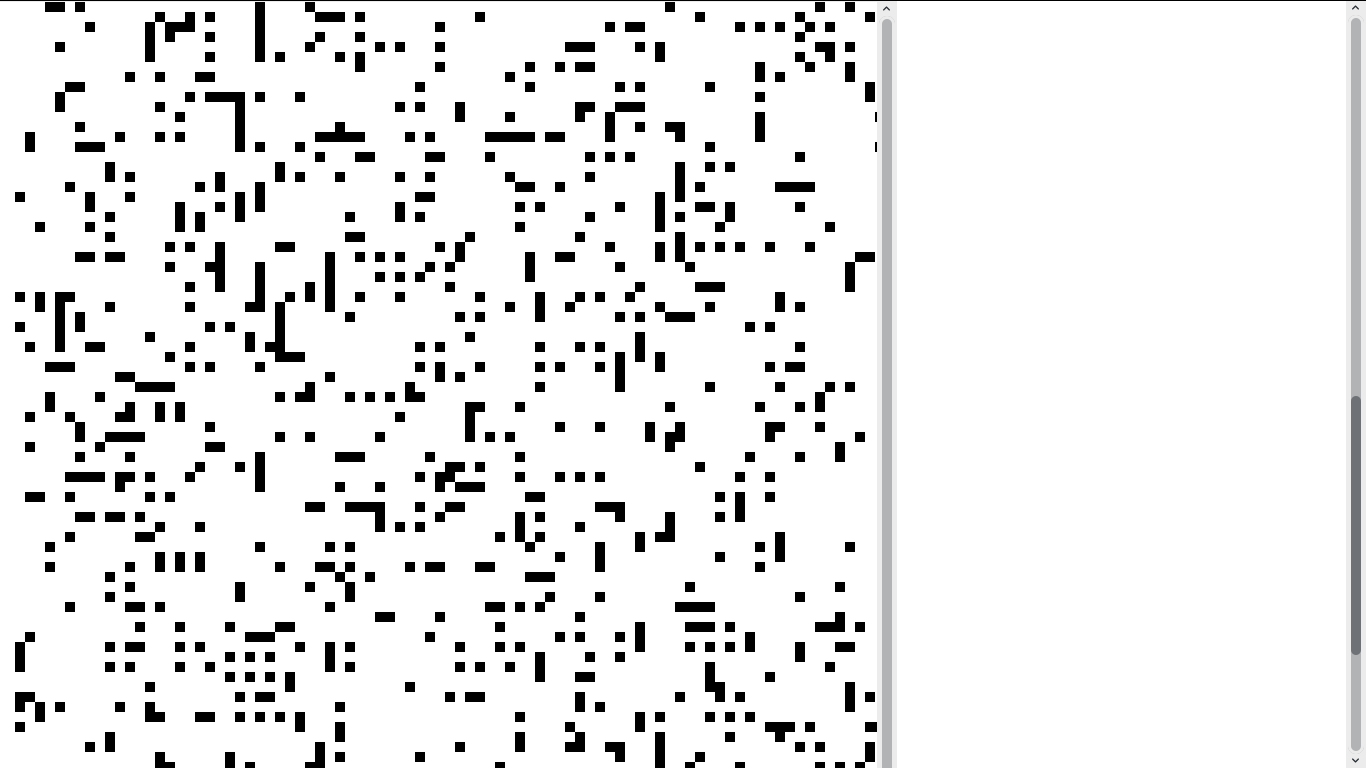
\includegraphics[width=15cm, height=8cm]{./img/3317-max-aux.png}
 \caption{Matriz auxiliar del autómata anterior}
 \label{fig:3317-max-aux}
\end{center}
\end{figure}

\begin{figure}[H]
\begin{center}
 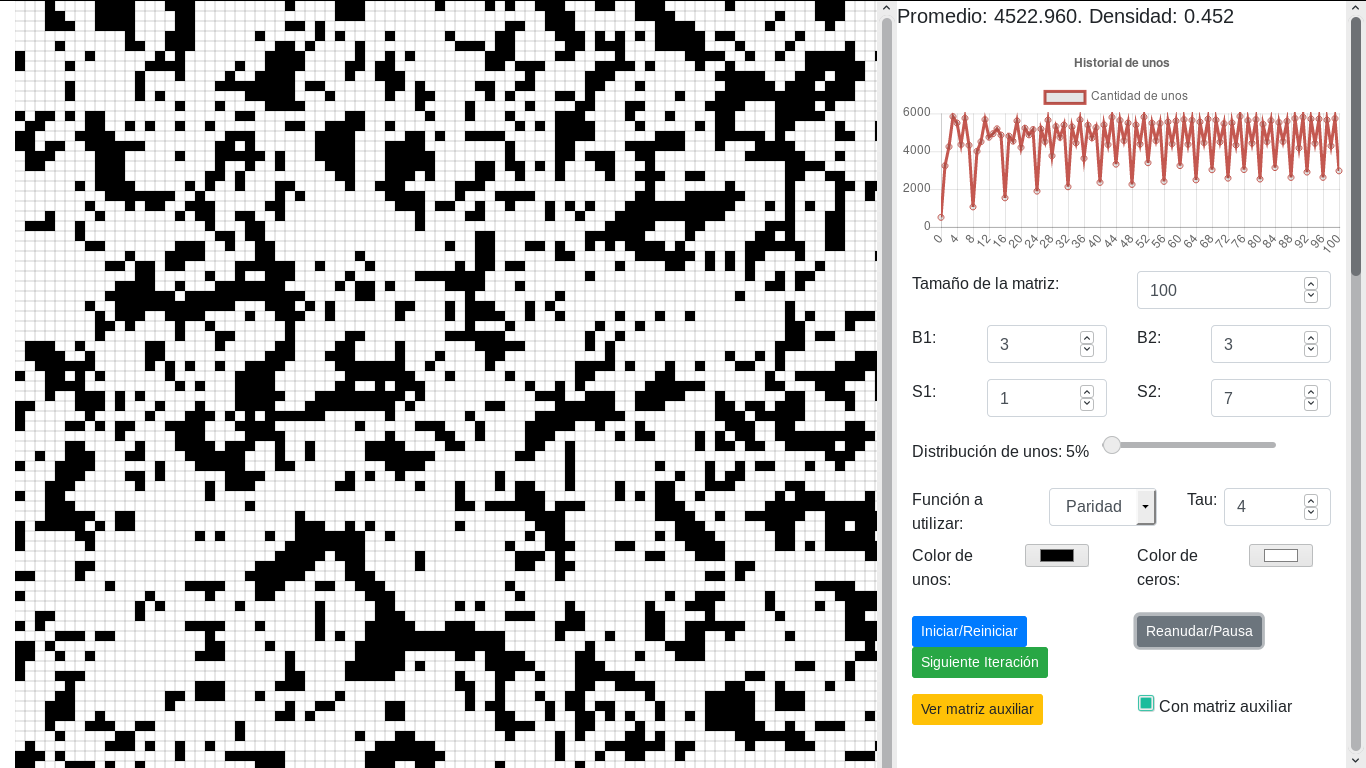
\includegraphics[width=15cm, height=8cm]{./img/3317-paridad.png}
 \caption{Utilizando la función de paridad}
 \label{fig:3317-paridad}
\end{center}
\end{figure}

\begin{figure}[H]
\begin{center}
 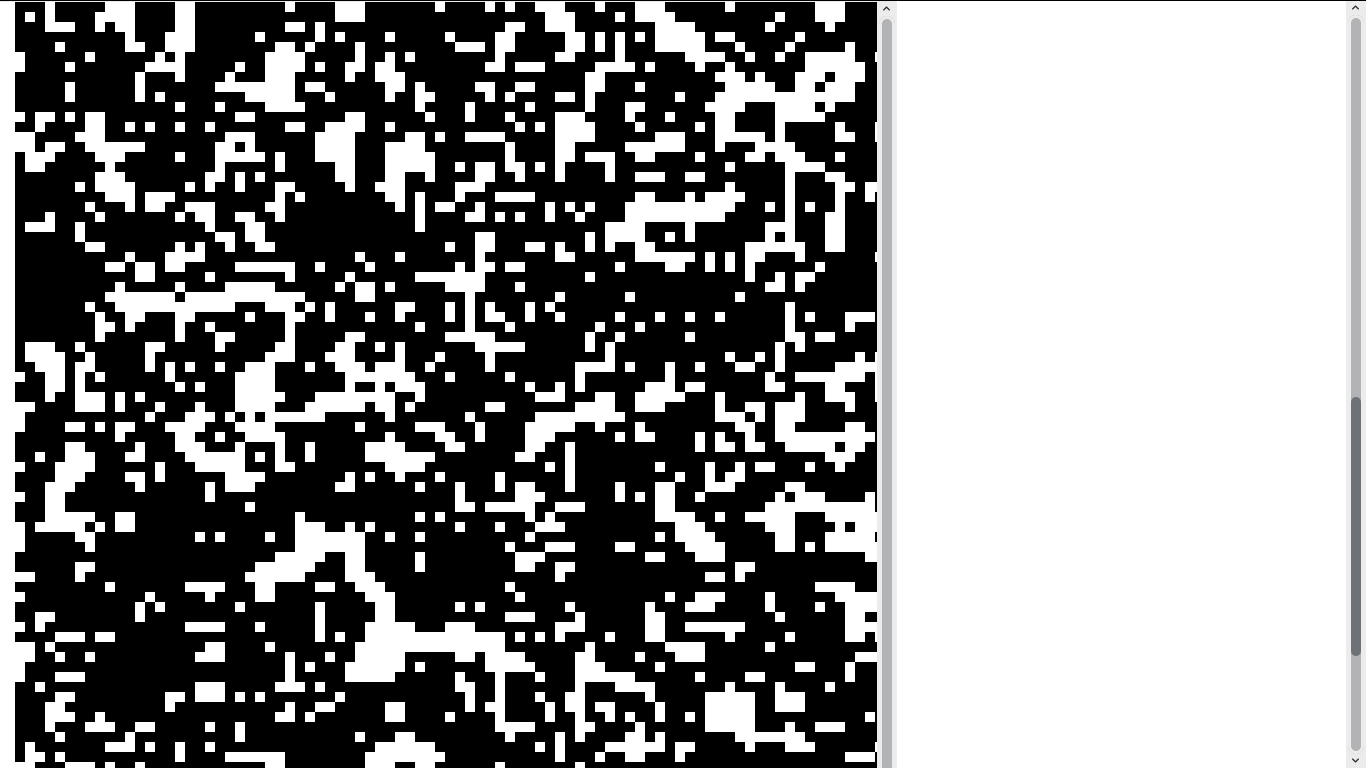
\includegraphics[width=15cm, height=8cm]{./img/3317-paridad-aux.png}
 \caption{Matriz auxiliar del autómata anterior}
 \label{fig:3317-paridad-aux}
\end{center}
\end{figure}
Con esta regla se tiene el comportamiento más raro al aplicar la regla de mínimo ya que la población aumenta en un inicio pero al final termina disminuyendo demasiado y estancarse en unos patrones en especifico.
\subsection{Regla: 2 3 3 6. Densidad: 10\%}

\begin{figure}[H]
\begin{center}
 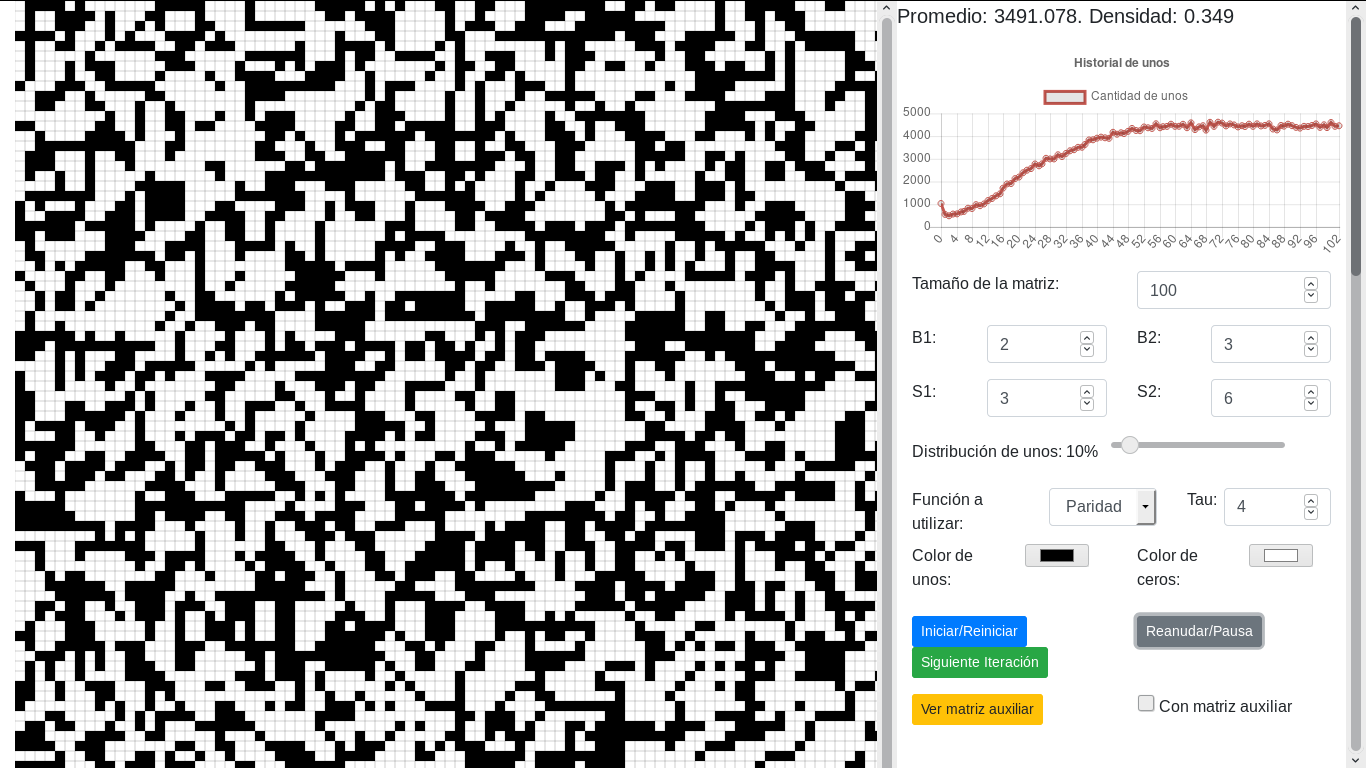
\includegraphics[width=15cm, height=8cm]{./img/2336.png}
 \caption{Resultado tras 100 iteraciones sin matriz auxiliar}
 \label{fig:2336}
\end{center}
\end{figure}

\begin{figure}[H]
\begin{center}
 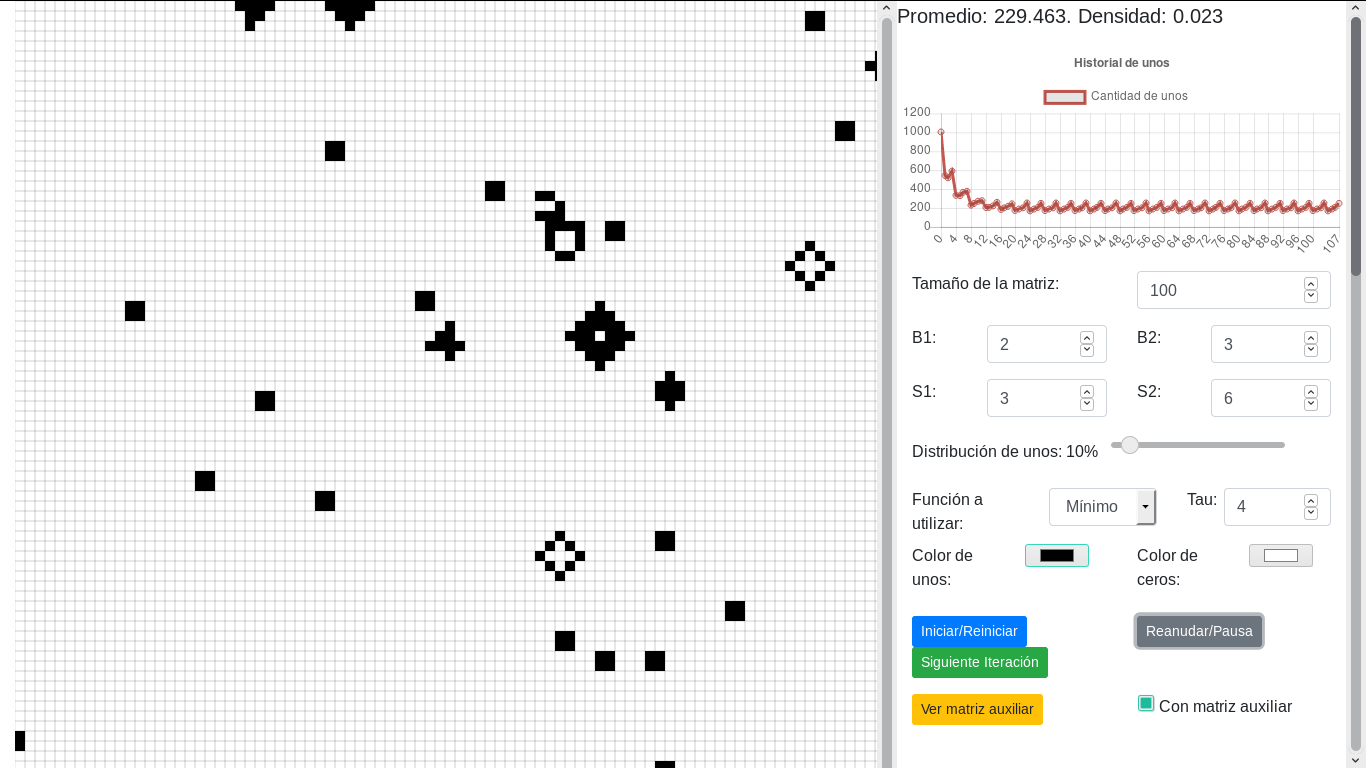
\includegraphics[width=15cm, height=8cm]{./img/2336-min.png}
 \caption{Utilizando la función de mínimo}
 \label{fig:2336-min}
\end{center}
\end{figure}

\begin{figure}[H]
\begin{center}
 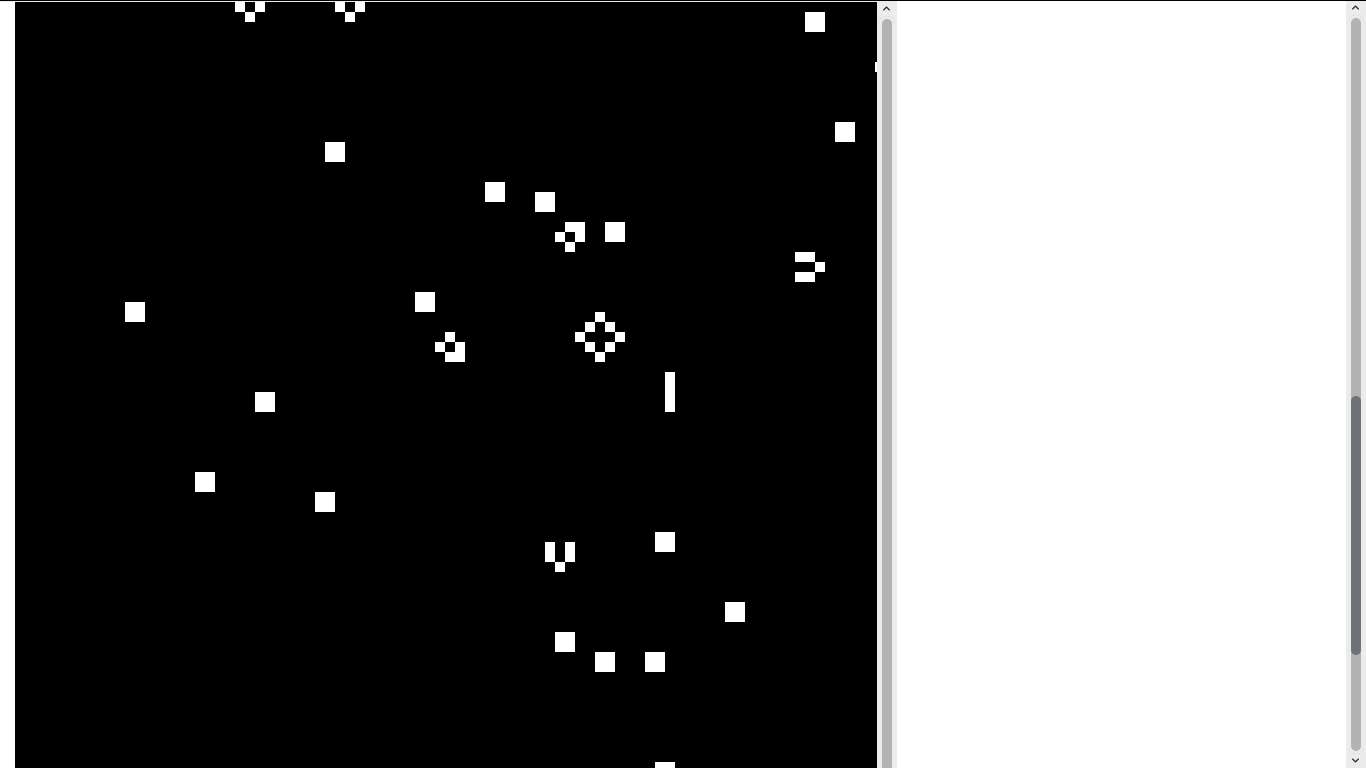
\includegraphics[width=15cm, height=8cm]{./img/2336-min-aux.png}
 \caption{Matriz auxiliar del autómata anterior}
 \label{fig:2336-min-aux}
\end{center}
\end{figure}

\begin{figure}[H]
\begin{center}
 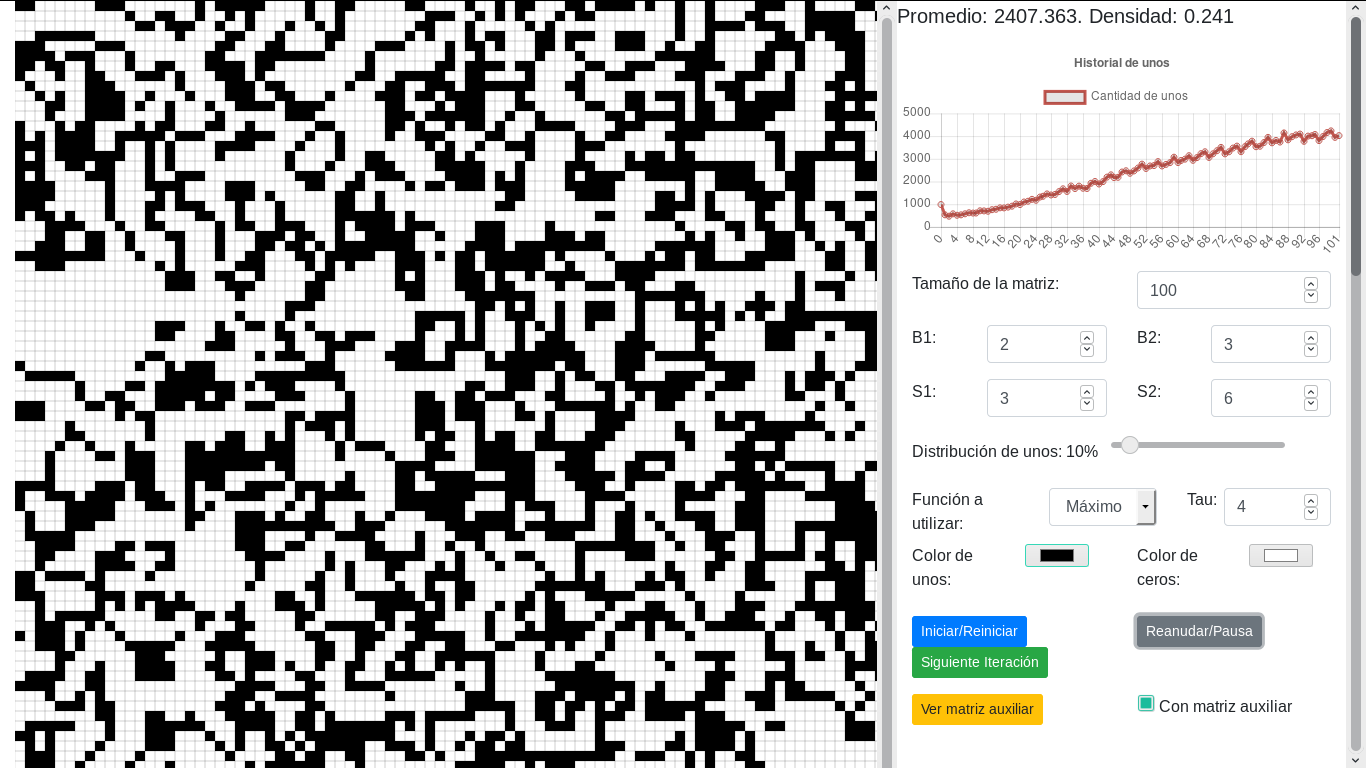
\includegraphics[width=15cm, height=8cm]{./img/2336-max.png}
 \caption{Utilizando la función de máximo}
 \label{fig:2336-max}
\end{center}
\end{figure}

\begin{figure}[H]
\begin{center}
 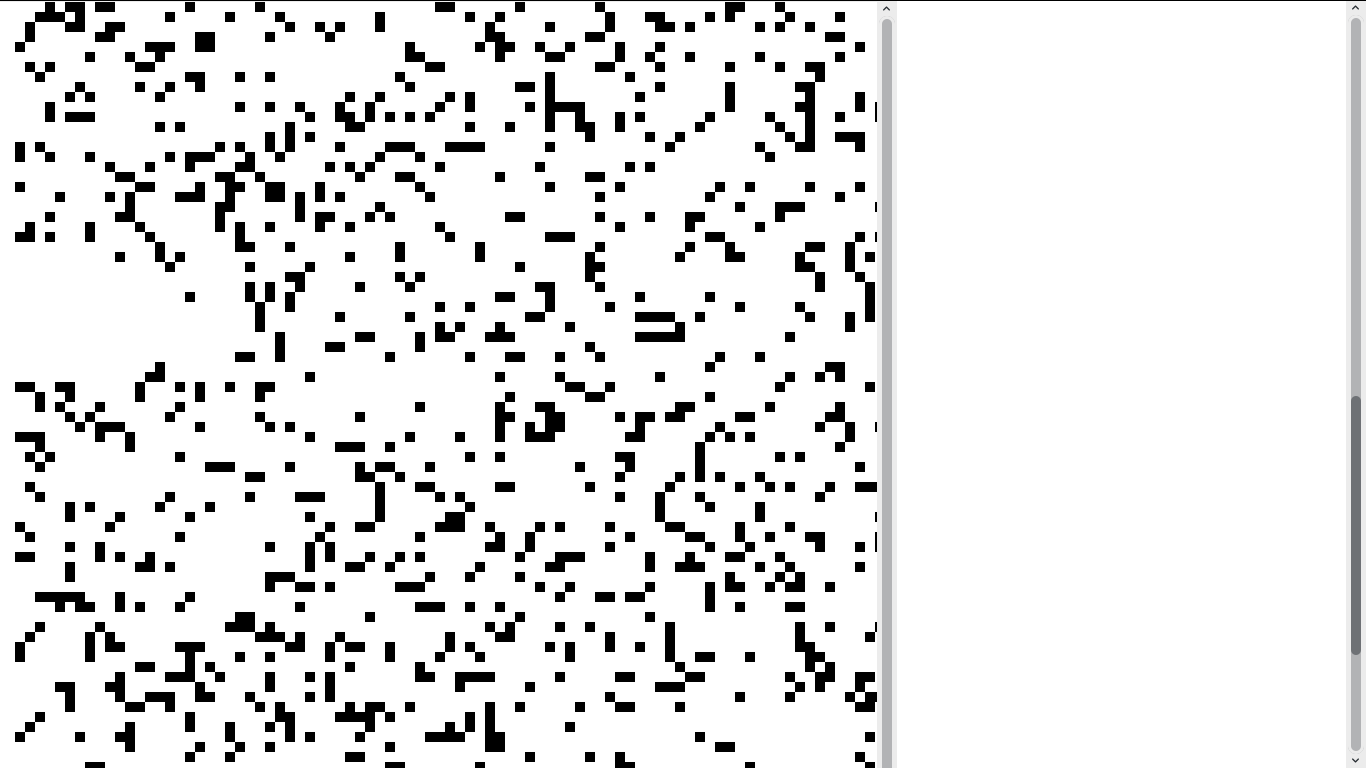
\includegraphics[width=15cm, height=8cm]{./img/2336-max-aux.png}
 \caption{Matriz auxiliar del autómata anterior}
 \label{fig:2336-max-aux}
\end{center}
\end{figure}

\begin{figure}[H]
\begin{center}
 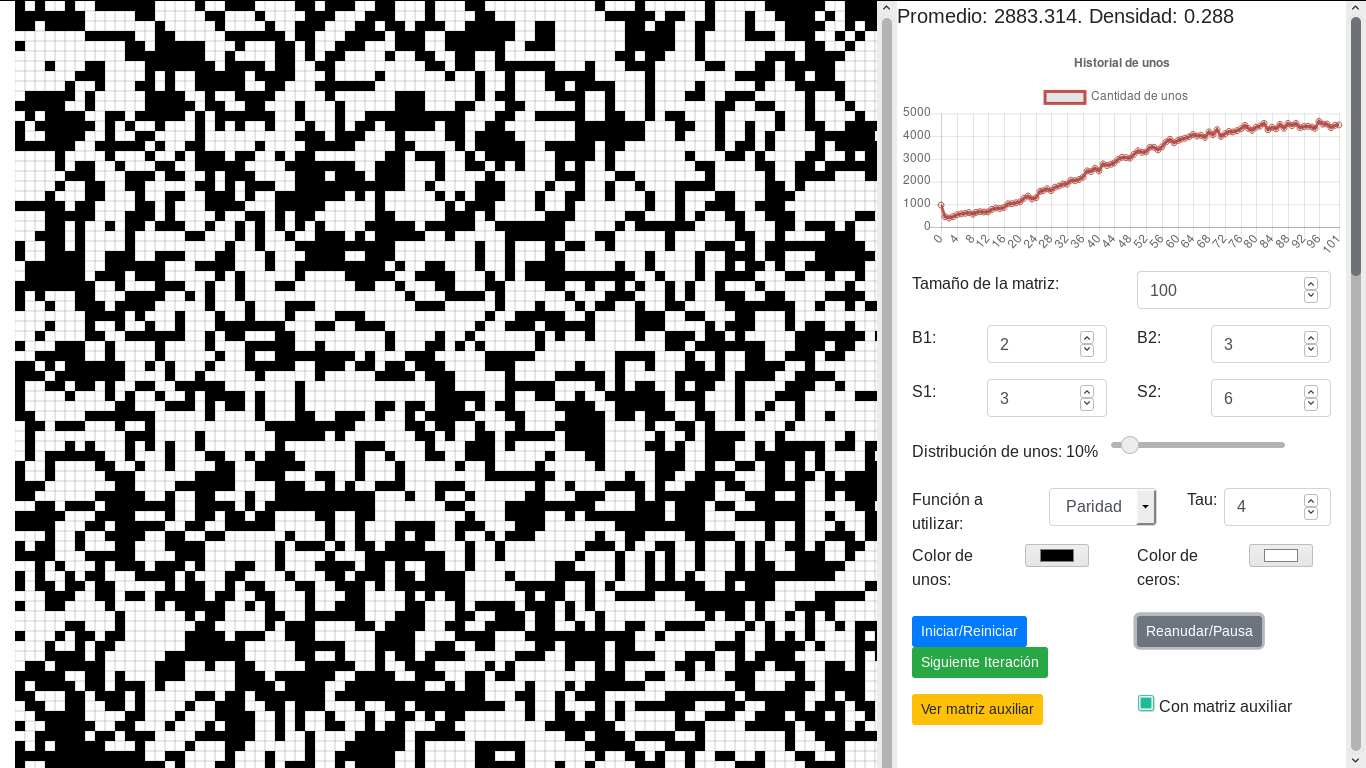
\includegraphics[width=15cm, height=8cm]{./img/2336-paridad.png}
 \caption{Utilizando la función de paridad}
 \label{fig:2336-paridad}
\end{center}
\end{figure}

\begin{figure}[H]
\begin{center}
 
\includegraphics[width=15cm, height=8cm]{./img/2336-paridad-aux.png}
 \caption{Matriz auxiliar del autómata anterior}
 \label{fig:2336-paridad-aux}
\end{center}
\end{figure}

Al igual que con la regla anterior, en esta regla se tiene el mismo comportamiento de disminución de la población al aplicar la regla de mínimo.

\subsection{Conclusiones}
El uso de una función y una matriz auxiliar para el calculo de las iteraciones en un autómata celular cambian el comportamiento de la función original, es decir, si se realiza la prueba y se compara la gráfica de unos de la regla del juego de la vida con y sin función auxiliar se puede apreciar que la que tiene la función auxiliar oscila con más frecuencia a diferencia de la que no utiliza una función extra, en esta la gráfica se estabiliza de una forma más rápida.

El uso de esta técnica al trabajar con autómatas celulares es bastante útil ya que permite el observar nuevos comportamientos con base a reglas ya conocidas, lo cual puede agilizar el estudio de estos modelos.

\bibliographystyle{ieeetr}
\bibliography{reporte}

\end{document}
